%%!TEX encoding = UTF-8 Unicode

% Several lines in file have comments suggesting common packages for the
% typical thesis in informatics or electronics developed at UA
% uncomment/comment the lines as required for your work
% Before each optional line you will have a small comment

% According to UA rules, font size should range from 10 to 12pt.
\documentclass[11pt,a4paper,openright,twoside,onecolumn]{memoir}

\listfiles
\fixpdflayout

\usepackage[utf8]{inputenc}

% Select Computer Modern Typewritter (For bold ttfamily in listings)
\usepackage{lmodern}
% OR... Bera Mono
%\usepackage[scaled]{beramono} % TTT Font
%\usepackage{anyfontsize} % As the name says...

\usepackage[T1]{fontenc}

% Enable for for Overleaf support
\usepackage{ifthen}
\def\useoverleaf{0}  % change to non-zero (for instance, 1) to enable it

\makeatletter
\newcommand{\makecoverfile}[0]{%
  \immediate\write18{latexmk -pdf cover.tex}%
}
\makeatother

% For PDF merging
\usepackage{pdfpages}

% Set DPI to 300
\pdfpxdimen=\dimexpr 1in/300\relax

% Allow the use of a larger number of packages
\usepackage{morewrites} 

% For English and Portuguese languages
% Portuguese will be the default.
% Uncomment \setlanguage below to change it
\usepackage[english,portuguese]{babel}

% Uncomment to use a custom date format
%\usepackage{datetime}
%\newdateformat{thesisdate}{\monthname[\THEMONTH] \THEYEAR} % Month Year

% Make pdf look better
\usepackage{microtype} 

% Uncomment to enable floats on facing pages
%\usepackage{dpfloat}

% Side by side figures
% Eg. Fig 1a, Fig 1b
\usepackage[hang,small,bf]{caption}
%\let\tion\undefined
%\let\subfloat\undefined
\usepackage{subcaption}

%\RequirePackage{textcase}

% Dropped Caps
%\usepackage{lettrine}

% Configure Hyperlink color
% As a matter or style, you may use this to enable/disable color boxes on links
%\usepackage[breaklinks=true,colorlinks=false,linkcolor=blue]{hyperref}
% Or use the default values provided by the hyperref package
\usepackage[hidelinks]{hyperref}

% Redefine section names according to your preference
%\def\sectionautorefname{Section}
%\def\chapterautorefname{Chapter}
%\def\figureautorefname{Figure}
%\def\listingautorefname{Listing}
%\def\tableautorefname{Table}

% Redefine code boxes
\ifthenelse{\equal{\useoverleaf}{0}}
{\usepackage[outputdir=build]{minted}}
{\usepackage{minted}}%

\addto\captionsportuguese{%
  \renewcommand\listingscaption{Código}
}
\fvset{fontsize=\footnotesize} % Make Code blocks smaller than text
\usepackage{csquotes}

% Add support for PDF Comments
\usepackage{comment}
\ifthenelse{\equal{\useoverleaf}{0}}
{\usepackage{pdfcomment}}{}
\usepackage{bookmark} % New Bookmarks

% For Multiple columns in Glossary
\usepackage{multicol}

% For Multiple rows in tables
\usepackage{multirow}

% Add support for Math symbols
\usepackage{amsmath}
\usepackage{amssymb}

% Add support for graphics
\usepackage{graphicx}

% Add support for Colors
\usepackage{xcolor}

% Add support for the Euro symbol
\usepackage{eurosym}

% Add support for missingfigure and todo
\usepackage{todonotes}

% Setup bibliography with Biber using IEEE style for proper UTF-8 support
\usepackage[backend=biber, style=ieee, sorting=none, natbib=true, mincitenames=1, maxcitenames=2]{biblatex}
\bibliography{bib/references.bib, bib/rfc.bib, bib/network.bib}

% Use acronyms
\usepackage[printonlyused]{acronym} % For acronyms

% Indenting the first paragraph after section start
\usepackage{indentfirst}

% For fixing listoflistings with memoir
\usepackage{xparse} 

% Uncomment the next lines to enable chart support through pgf and tikz
% This may require you to install further packages in your Tex system
%\usepackage[version=0.96]{pgf}
%\usepackage{tikz}

% UML support
%\usepackage{pgf-umlsd}

% Trees, Arrows, Mindmaps and other popular objects
%\usetikzlibrary{arrows,shadows,trees,shapes,decorations,automata,backgrounds,petri,mindmap} % for pgf-umlsd

% Package to master SI units
\usepackage[detect-weight=true, binary-units=true]{siunitx}
% For Electric Circuits
%\sisetup{load-configurations = binary}

% Set Voltage direction accordingly
% Option : oldvoltagedirection,nooldvoltagedirection,RPvoltages,EFvoltages
% More information at: https://mirrors.ibiblio.org/CTAN/graphics/pgf/contrib/circuitikz/doc/circuitikzmanual.pdf
% By default this template is using the Old Voltage Direction
%\usepackage[oldvoltagedirection,american,cuteinductors,smartlabels]{circuitikz}
%\usetikzlibrary{calc}
%\ctikzset{bipoles/thickness=1}
%\ctikzset{bipoles/length=0.8cm}
%\ctikzset{bipoles/diode/height=.375}
%\ctikzset{bipoles/diode/width=.3}
%\ctikzset{tripoles/thyristor/height=.8}
%\ctikzset{tripoles/thyristor/width=1}
%\ctikzset{bipoles/vsourceam/height/.initial=.7}
%\ctikzset{bipoles/vsourceam/width/.initial=.7}
%\tikzstyle{every node}=[font=\small]
%\tikzstyle{every path}=[line width=0.8pt,line cap=round,line join=round]

% For inline TT text (e.g. code snippets)
\usepackage{verbatim}

% Frames around figures and allow force placement
\usepackage{float}

% Configure Float style
%\floatstyle{boxed}
%\restylefloat{table}
%\restylefloat{figure}
%\restylefloat{lstlisting}

% For test purposes you may use the lipsum package to create dummy text
\usepackage{lipsum} % REMOVE

%Keep floats inside section!
\usepackage[section]{placeins}
\let \oldsubsubsection \subsubsection
\renewcommand{\subsubsection}[2][]{
  \FloatBarrier
  \oldsubsubsection#1{#2}
}
\let \oldsubsection \subsection
\renewcommand{\subsection}[2][]{
  \FloatBarrier
  \oldsubsection#1{#2}
}
\let \oldsection \section
\renewcommand{\section}[2][]{
  \FloatBarrier
  \oldsection#1{#2}
}
\let \oldchapter \chapter
\renewcommand{\chapter}[2][]{
  \FloatBarrier
  \oldchapter#1{#2}
}



% Use the built-in division styling
\headstyles{memman}

% Include subsections in the TOC
\settocdepth{subsection}

% Numbering down to subsections as well
\setsecnumdepth{subsection}

% extra index for first lines
\makeindex[lines]

% Margins for University of Aveiro Thesis
\setlrmarginsandblock{3cm}{2.5cm}{*}
\setulmarginsandblock{3cm}{3cm}{*}
\checkandfixthelayout

% Or select your custom spacing to make any ajustment
%\addtolength{\parskip}{0.5\baselineskip}
\linespread{1.5}

\newcommand\mainmatterWithoutReset
{\edef\temppagenumber{\arabic{page}}%
  \mainmatter
  \setcounter{page}{\temppagenumber}%
}


%%%%%%%%%%%%%%%%%%%%%%%%%%%%%%%%%%%%%%%%%%%%%%%%%%
% Document begins here
%%%%%%%%%%%%%%%%%%%%%%%%%%%%%%%%%%%%%%%%%%%%%%%%%%

\begin{document}

% Fix the numbering scheme by having a ghost style for page numbering
\pagenumbering{Alph}

\ifthenelse{\equal{\useoverleaf}{0}}{}{\makecoverfile{}}%
\includepdf[pages=-]{cover.pdf}

% Uncomment to enable English
\selectlanguage{english}


% Front matter

%Custom Chapter style named `thesis`
\makechapterstyle{thesis}{% Based on ell
  \chapterstyle{default}
  \renewcommand*{\chapnumfont}{\normalfont\sffamily}
  \renewcommand*{\chaptitlefont}{\normalfont\Huge\sffamily}
  \settowidth{\chapindent}{\chapnumfont 111}
  \renewcommand*{\chapterheadstart}{\begingroup
    \vspace*{\beforechapskip}%
    \begin{adjustwidth}{}{-\chapindent}%
    \hrulefill
    \smash{\rule{0.4pt}{15mm}}
    \end{adjustwidth}\endgroup}
  \renewcommand*{\printchaptername}{}
  \renewcommand*{\chapternamenum}{}
  \renewcommand*{\printchapternum}{%
    \begin{adjustwidth}{}{-\chapindent}
    \hfill
    \raisebox{10mm}[0pt][0pt]{\fontsize{30}{25}\selectfont\chapnumfont \thechapter}%
                              \hspace*{1em}
    \end{adjustwidth}\vspace*{-3.0\onelineskip}}
  \renewcommand*{\printchaptertitle}[1]{%
    \vskip\onelineskip
    \raggedleft {\chaptitlefont ##1}\par\nobreak\vskip 4\onelineskip}}


% Select chapter style from existing or select custom
%\chapterstyle{thesis} % Others: dowding, demo2, dash, chappell, brotherton, bianchi, ger, madsen, tatcher, veelo,indexes)
% thesis can also be used as defined previously
% Check the memoir documentation for the available themes
% Default is veelo
\chapterstyle{veelo}
\makeoddfoot{plain}{}{\thepage}{} % Added by André Zúquete to fix a page numbering issue on the veelo chapter style


% If you feel adventurous you can also define all aspects of your theme
% Use either this input or the chapterstyle before
% % Rules
\newcommand{\thinRule}{\rule{\textwidth}{0.25pt}}

% Customize heading appearances
% Define styles
\newcommand{\partSize}{\Huge}
\newcommand{\partStyle}{\lsstyle\scshape}
\newcommand{\chapterSize}{\Huge}
\newcommand{\chapterStyle}{\lsstyle\scshape}
\newcommand{\chapterAfter}{}
\newcommand{\sectionSize}{\Large}
\newcommand{\sectionStyle}{\scshape\MakeTextLowercase}
\newcommand{\subsectionSize}{\large}
\newcommand{\subsectionStyle}{\scshape\MakeTextLowercase}
\newcommand{\subsubsectionSize}{\large}
\newcommand{\subsubsectionStyle}{\scshape\MakeTextLowercase}
\newlength{\partNumSizePt}
\setlength{\partNumSizePt}{60pt}
\newlength{\chapterNumSizePt}
\setlength{\chapterNumSizePt}{60pt}
\newcommand{\partNumSize}{%
  \fontsize{\partNumSizePt}{1.2\partNumSizePt}\selectfont%
}
\newcommand{\partNumStyle}{\partChapterNumColor}
\newcommand{\chapterNumSize}{%
  \fontsize{\chapterNumSizePt}{1.2\chapterNumSizePt}\selectfont%
}
\newcommand{\chapterNumStyle}{\partChapterNumColor}

% Customize parts
\renewcommand{\partnamefont}{\partSize\partStyle}
\renewcommand{\partnumfont}{\partNumSize\partNumStyle}
\renewcommand{\printpartname}{}
\renewcommand{\printparttitle}[1]{%
  \normalfont\normalcolor\partnamefont #1
}

% Customize chapters
\makeatletter
\setlength{\beforechapskip}{30pt}
\renewcommand*{\chapterheadstart}{\vspace*{\beforechapskip}}
\setlength{\afterchapskip}{3ex}
\setlength{\midchapskip}{3ex}
\renewcommand*{\chapnamefont}{%
  \Large\flushright\chapterStyle\partChapterNumColor%
}
\renewcommand*{\chapnumfont}{\chapterNumSize\chapterNumStyle}
\renewcommand*{\chaptitlefont}{%
  \normalfont\flushleft\normalcolor\chapterSize\chapterStyle%
}
\renewcommand*{\printchaptername}{%
  \chapnamefont\MakeTextLowercase{\@chapapp}%
}
\renewcommand*{\chapternamenum}{\quad}
\renewcommand*{\printchapternum}{%
%  \chapnumfont\textls[-75]{\classicstylenums{\thechapter}}%
 \chapnumfont\textls[-75]{\thechapter}%

}
\renewcommand*{\printchaptertitle}[1]{%
  \chaptitlefont #1
  \chapterAfter
}
\makeatother
% Customize sections and subsections
\setsecnumformat{\csname my#1\endcsname\quad}
\setsecheadstyle{\sectionSize\sectionStyle}
\newcommand{\mysection}{{\thesection}}
\setlength{\beforesecskip}{3em}


\setsubsecheadstyle{\subsectionSize\subsectionStyle}
\newcommand{\mysubsection}{{\normalfont\subsectionSize\thesubsection}}
\setlength{\beforesubsecskip}{3em}

\setsubsubsecheadstyle{\subsubsectionSize\subsubsectionStyle}
\newcommand{\mysubsubsection}{{\normalfont\subsubsectionSize\thesubsubsection}}
\setlength{\beforesubsubsecskip}{2em}

% Customize "Table of ..." appearance
% Customize headings
\newcommand{\renewPrintXTitle}[1]{%
  \renewcommand{#1}[1]{%
    \printchaptertitle{##1}%
  }%
}
\renewPrintXTitle{\printtoctitle}
\renewPrintXTitle{\printlottitle}
\renewPrintXTitle{\printloftitle}

% Customize ToC headings
\renewcommand{\cftpartfont}{\partChapterNumColor\partStyle}
\renewcommand{\cftchapterfont}{\chapterStyle}
\renewcommand{\cftsectionfont}{}
\renewcommand{\cftsubsectionfont}{}
\renewcommand{\cftfigurefont}{}
\renewcommand{\cfttablefont}{}
\newcommand{\cftlstlistingfont}{}

% Increase number width
\newlength{\cftNumWidthIncrease}
\setlength{\cftNumWidthIncrease}{0.25em}
\addtolength{\cftpartnumwidth}{\cftNumWidthIncrease}
\addtolength{\cftchapternumwidth}{\cftNumWidthIncrease}
\addtolength{\cftsectionindent}{\cftNumWidthIncrease}
\addtolength{\cftsubsectionindent}{\cftNumWidthIncrease}
% No leader dots
%\renewcommand*{\cftpartdotsep}{\cftnodots}
%\renewcommand*{\cftchapterdotsep}{\cftnodots}
%\renewcommand*{\cftsectiondotsep}{\cftnodots}
%\renewcommand*{\cftsubsectiondotsep}{\cftnodots}
%\renewcommand*{\cftfiguredotsep}{\cftnodots}
%\renewcommand*{\cfttabledotsep}{\cftnodots}
%\newcommand*{\cftlstlistingdotsep}{\cftnodots}
% Set page numbers immediately after entry text
\newcommand{\tocEntryPageSep}{\hspace{1em}}
\renewcommand{\cftpartleader}{\cftdotfill{\cftdotsep}}
%\renewcommand{\cftpartafterpnum}{\cftparfillskip}
%\renewcommand{\cftchapterleader}{\tocEntryPageSep}
\renewcommand{\cftchapterleader}{\cftdotfill{\cftdotsep}}
%\renewcommand{\cftchapterafterpnum}{\cftparfillskip}
\renewcommand{\cftsectionleader}{\cftdotfill{\cftdotsep}}
%\renewcommand{\cftsectionafterpnum}{\cftparfillskip}
\renewcommand{\cftsubsectionleader}{\cftdotfill{\cftdotsep}}
%\renewcommand{\cftsubsectionafterpnum}{\cftparfillskip}
\renewcommand{\cftfigureleader}{\cftdotfill{\cftdotsep}}
%\renewcommand{\cftfigureafterpnum}{\cftparfillskip}
\renewcommand{\cfttableleader}{\cftdotfill{\cftdotsep}}
%\renewcommand{\cfttableafterpnum}{\cftparfillskip}
\newcommand{\cftlstlistingleader}{\cftdotfill{\cftdotsep}}
%\newcommand{\cftlstlistingafterpnum}{\cftparfillskip}
% Customize page numbers
\newcommand{\tocPageStyle}{\tocPageColor}
\renewcommand{\cftpartpagefont}{\tocPageStyle}
\renewcommand{\cftchapterpagefont}{\tocPageStyle}
\renewcommand{\cftsectionpagefont}{\tocPageStyle}
\renewcommand{\cftsubsectionpagefont}{\tocPageStyle}
\renewcommand{\cftfigurepagefont}{\tocPageStyle}
\renewcommand{\cfttablepagefont}{\tocPageStyle}
\newcommand{\cftlstlistingpagefont}{\tocPageStyle}

% Abstract
% Remove indents around abstract text
\setlength{\absleftindent}{0pt}
\setlength{\absrightindent}{0pt}
% Change font size to conform with the rest of the document text
\renewcommand{\abstracttextfont}{\normalsize}

% Customize headers and footers including page numbers
\newcommand{\hfTextSize}{\footnotesize}
\newcommand{\headTextStyle}{\lsstyle\scshape\MakeTextLowercase}
\nouppercaseheads
\makeevenhead{headings}%
             {\hfTextSize\thepage}%
             {}%
             {\hfTextSize\headTextStyle\leftmark}
\makeevenhead{plain}%
             {\hfTextSize\thepage}%
             {}%
             {\hfTextSize\headTextStyle\leftmark}
\makeoddhead{headings}%
            {\hfTextSize\headTextStyle\rightmark}%
            {}%
            {\hfTextSize\thepage}
\makeoddhead{plain}%
            {\hfTextSize\headTextStyle\rightmark}%
            {}%
            {\hfTextSize\thepage}


% Customize captions
\newcommand{\captionSize}{\small}
\newcommand{\captionStyle}{\scshape}
\newcommand{\captionWidthRatio}{0.9}

\captionnamefont{\captionSize\captionStyle}
\captiontitlefont{\captionSize}
\captiondelim{ -- }
\captiontitlefinal{}
\changecaptionwidth
%\captionwidth{\captionWidthRatio\textwidth}

% Define colors
%\newcommand{\titleColor}{\color[rgb]{0.616, 0.0627, 0.176}}
\newcommand{\titleColor}{\color[rgb]{0,0,0}}

\newcommand{\partChapterNumColor}{\titleColor}
\newcommand{\dropCapColor}{\titleColor}
%\newcommand{\tocPageColor}{\color[rgb]{0.0980, 0.329, 0.651}}

\newcommand{\tocPageColor}{\color[rgb]{0, 0,0}}
\definecolor{shade0}{rgb}{1.0 , 1.0 , 1.0 }
\definecolor{shade1}{rgb}{0.9 , 0.9 , 0.9 }
\definecolor{shade2}{rgb}{0.8 , 0.8 , 0.8 }
\definecolor{shade3}{rgb}{0.65, 0.65, 0.65}
\definecolor{shade4}{rgb}{0.45, 0.45, 0.45}
\definecolor{shade5}{rgb}{0.0 , 0.0 , 0.0 }



%Exclude sub figures from List of Figures
%\captionsetup[subfloat]{list=no}

% Texts
\newenvironment{introduction}
{%
  \begin{minipage}{\textwidth}%
   \itshape%
}
{%
  \end{minipage}%
  \par\addvspace{2\baselineskip plus 0.2\baselineskip minus 0.2\baselineskip}%
}

% Select Page style
\pagestyle{plain}


\frontmatter

\tightlists
\midsloppy
\raggedbottom

\setcounter{tocdepth}{2} %subsections are added to the TOC
\setcounter{secnumdepth}{4} %subsubsections are numbered

% Initial document tables start here: TOC, LOF, LOT, Glossary
% Table of contents with slightly smaller font
\cleardoublepage
{\small\tableofcontents}

% List of figures with slightly smaller font
\cleardoublepage
{\small\listoffigures}

% List of tables with slightly smaller font
\cleardoublepage
{\small\listoftables}

% List of code snippets

% Fix for Listings with memoir

% \RenewDocumentCommand \chapter { s O{#3} m }{%
%   \FloatBarrier
%   \IfValueTF{#1}  % if optional star is seen
%     {\oldchapter*{#2}}
%     {\oldchapter#1{#2}}
% }

% \renewcommand{\listingscaption}{Código}
% \renewcommand{\listoflistingscaption}{Lista de Excertos de Código}
% \cleardoublepage
% {\small\listoflistings}
% \addcontentsline{toc}{chapter}{\listoflistingscaption}

% Reset Chapters
\renewcommand{\chapter}[2][]{
  \FloatBarrier
  \oldchapter#1{#2}
}

% Print Glossary
{\small\chapter{Glossário}

\footnotesize
\SingleSpacing

\begin{multicols}{2}
\begin{acronym}[AAAAAA]

	\acro{ict}[ICT]{Information and Communication Technology}
	\acro{isp}[ISP]{Internet Service Provider}
	\acro{dsl}[DSL]{Digital Subscriber Line}
	\acro{adsl}[ADSL]{Asymmetric Digital Subscriber Line}
	\acro{docsis}[DOCSIS]{Data Over Cable Service Interface Specification}
	\acro{epon}[EPON]{Ethernet Passive Optical Network}
	\acro{wdm}[WDM]{Wavelength Division Multiplexing}
	\acro{oxc}[OXC]{Optical Cross-Connect}
	\acro{tcp}[TCP]{Transmission Control Protocol}
	\acro{ip}[IP]{Internet Protocol}
	\acro{cpe}[CPE]{Customer Premises Equipment}
	\acro{watt}[W]{Watt}
	\acro{kilowatt-hour}[kWh]{Kilowatt-hour}
	\acro{gigabyte}[GB]{Gigabyte}
	\acro{lan}[LAN]{Local Area Network}
	\acro{wan}[WAN]{Wide Area Network}
	\acro{wpan}[WPAN]{Wireless Personal Area Network}
	\acro{wlan}[WLAN]{Wireless Local Area Network}
	\acro{wman}[WMAN]{Wireless Metropolitan Area Network}
	\acro{wwan}[WWAN]{Wireless Wide Area Network}

\end{acronym}
\end{multicols}

}

%%%%%%%%%%%%%%%%%%%%%%%%%%%%%%%%%%%%%%%%%%%%%%%%%%%%%%%
% Main document starts here
%%%%%%%%%%%%%%%%%%%%%%%%%%%%%%%%%%%%%%%%%%%%%%%%%%%%%%%

\mainmatter

% Line spacing: 1.5 pt 
\OnehalfSpacing

%%%%%%%%%%%%%%%%%%%%%%%%%%%%%%%%%%%%%%%%%%%%%%%%%%%%%%%
% Start of Thesis text 
%%%%%%%%%%%%%%%%%%%%%%%%%%%%%%%%%%%%%%%%%%%%%%%%%%%%%%%

% Uncomment to add further chapters
%

\chapter{Introdução}
\label{chapter:introduction}

\begin{introduction}
A short description of the chapter.

A memorable quote can also be used.
\end{introduction}



\section{Acrónimos}

Primeira e seguintes referências: \ac{h2o}, \ac{h2o}

Plural, acrónimo expandido e curto: \acp{h2o}, \acs{h2o}, \acl{h2o}

Com citação\footnote{Necessária entrada na bibliografia}: \ac{adsl}, \ac{adsl}


\section{Fontes}

\begin{itemize}
\item{\tiny Tiny}
\item{\scriptsize Scriptsize}
\item{\footnotesize Footnotes}
\item{\small Small}
\item{\normalsize Normal}
\item{\large large}
\item{\Large Large}
\item{\LARGE LARGE}
\item{\huge huge}
\item{\Huge Huge}
\end{itemize}

\section{Unidades}

Utilizando o pacote \verb|siunitx| é possível utilizar unidades do Sistema Internacional. Exemplo: a aceleração da gravidade é de \SI{9.8}{\metre\per\second\squared} e um ficheiro ocupa \SI{1}{\mebi\byte}. 

\section{Code Blocks}
%\lipsum[5]
Uma listagem pode ser apresentada com o ambiente \texttt{listing}, que é um float (objeto flutuante, tal como uma figura ou uma tabela).

A listagem em Código~\ref{lbl:snippet-test} mostra um exemplo em C.

\begin{listing}[h]
\begin{minted}{c}

#include <stdio.h>
#define N 10
/* Block
 * comment */
 
int main()
{
    int i;
 
    // Line comment.
    puts("Hello world!");
 
    for (i = 0; i < N; i++)
    {
        puts("LaTeX is also great for programmers!");
    }
 
    return 0;
}
\end{minted}
\caption{This caption appears below the code.}
\label{lbl:snippet-test}
\end{listing}

%\lipsum[5]

\section{Citações}

Algumas formas distintas de citar:

\begin{itemize}
    \item \textbf{Apenas referência}:~\cite{rfc44}
    \item \textbf{Apenas data}:~\citedate{rfc44}
    \item \textbf{Apenas ano}:~\citeyear{rfc44}
    \item \textbf{Apenas autor}:~\citeauthor{rfc44}
    \item \textbf{Apenas editor}:\citelist{rfc44}{organization}
    \item \textbf{Autor e referência}:\citet{rfc44}
\end{itemize}



\chapter{Introduction}
\label{chapter:introduction}

\begin{introduction}

Energy consumption has been a topic of discussion lately due to the increase of global warming. The \ac{ict} sector is responsible for around 4-6\% of the global eletricity use in 2020 \citet{UK-parliament}. The main contributer to the energy consumption of the \ac{ict} sector are datacenters, which account for XXX\% (\citet{check source}). With the increase of internet use and the need to process large amounts of data, the energy consumption of the \ac{ict} sector will only increase further.

The primary objective of this thesis is to analyse data compression algorithms and their impact on the energy consumption of the \ac{ict} sector.
To achieve this objective, a model of the energy consumption of the \ac{ict} sector was develop, along side a web calculator to compare different compression algorithms on several uses cases. 

In this chapter, we will present reasearch questions, followed by the hypotheses and objectives of the thesis. We will then present the risk assessment and impact of the thesis, concluding with the contributions of the thesis. 

\end{introduction}

\section{Researh questions}

To define the scope of the thesis, the following research questions were defined:

- What is the system boundary of the model?

- How to test the accuracy of the model?

- What is the impact of each component of the model?

\section{Hypotheses}

\section{Objectives}

- Study the current energy models of the internet

- Develop an aggregated model.

- Develop a web calculator to show the model

- Create case studies to benchmark the model


\section{Risk assessment and impact}

\section{Contributions}

\section{Thesis structure}

This thesis is divided into 6 chapters. After this introduction (chapter 1), a background on the concepts covered, such as network structure and compressions, is presented in chapter 2. Chapter 3 focuses on the recent works that have modeled part of the internet. An aggregation of these recent models will be presented in chapter 4. Chapter 5 will present the web calculator developed to show the model, along side with use cases on how to use the web calculator. Finally, chapter 6 will present the conclusions of the thesis and future work.


% - chapter 1: introduction
% - chapter 2: background
% - chapter 3: related work
% - chapter 4: Energy model
% - chapter 5: web calculator and use cases
% - chapter 7: conclusion


\chapter{Background}
\label{chapter:background}

\begin{introduction}
    
    The modelling of the energy consumption of the \ac{ict} sector is a complex task, because it involves modelling several systems, each with their distinct topologies and external factors.

    In this chapter we can find a description of the topology of the different systems that comprise the \ac{ict} sector and a highlight on the main component of each system. Moreover, the chapter also includes a description on the basics of compression algorithms and the different types of compression algorithms.

\end{introduction}

\section{System Boundaries}
\label{section:system_boundaries}

The definition of system boundaries is an important factor in the modelling of energy consumption. As seen in the compilation of studies made by \citet{Aslan2018}, the system boundaries are one of the main factors for the discrepancies of the results.

The common consensus is that the system boundaries for the model of the internet should exclude datacenters and user devices, as shown by \citet{Coroama2014}. Our study however won't be modeling only the internet but also the impact on datacenters and of the compression/decompression algorithm in the end user device. So the overall system boundary will include all the \ac{ict} sector. 

So our study divides the system boundary in three main components: the network, datacenters and the end user devices (Figure \ref{figure:system_boundaries}). The network is divided in three main components: \ac{cpe}, Access Network and Core Network. The datacenter is also divided in three components: Servers, Storage and Datacenter Network. Lastly the end user devices only includes the compression/decompression algorithm cost. 

\begin{figure}[h]
    \centering
    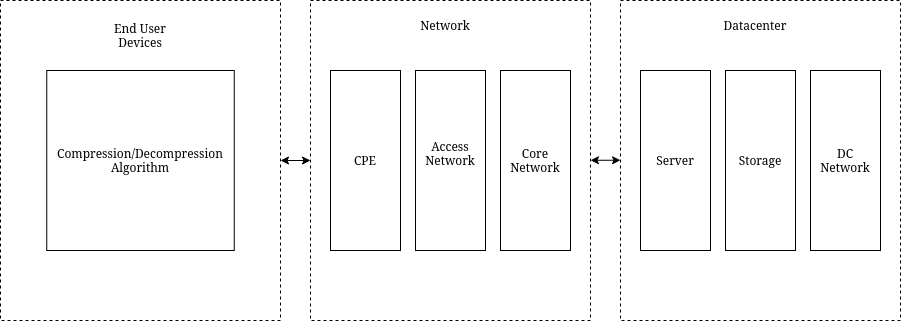
\includegraphics[width=1\textwidth]{figs/System_Boundary.png}
    \caption{Complete system boundary of the model and subsystem of each component.}
    \label{figure:system_boundaries}
\end{figure}

\section{Internet}

The internet is the most complex component of the model.
Internet started has an interconnection of a small number of local university networks, which were composed of a few routers and cables. Nowadays, the internet is a global network of networks, composed of millions of routers, switches and cables, that interconnects billions of end users. This communication is made possible by the use of the \ac{tcp} and \ac{ip} protocols.

Because of its complexity the system is usually divided into smaller components. However, the delimitation on where each component begins and ends can vary from paper to paper. In this thesis, we use the delimitation proposed by \citet{Coroama2015} and \citet{Schien2015}, which divides the internet in four main components: \ac{cpe}, access network, \ac{ip} core network and undersea cables.

\subsection{\acl{cpe} and Access Network}

There are several technologies used to connect the user to the Ethernet. They can be either wired or wireless and can be part of the \ac{cpe} layer or access network layer. Figure \ref{figure:network_technologies} highlights which technologies are currently used and in what layer they belong to.

\begin{figure}[h]
    \centering
    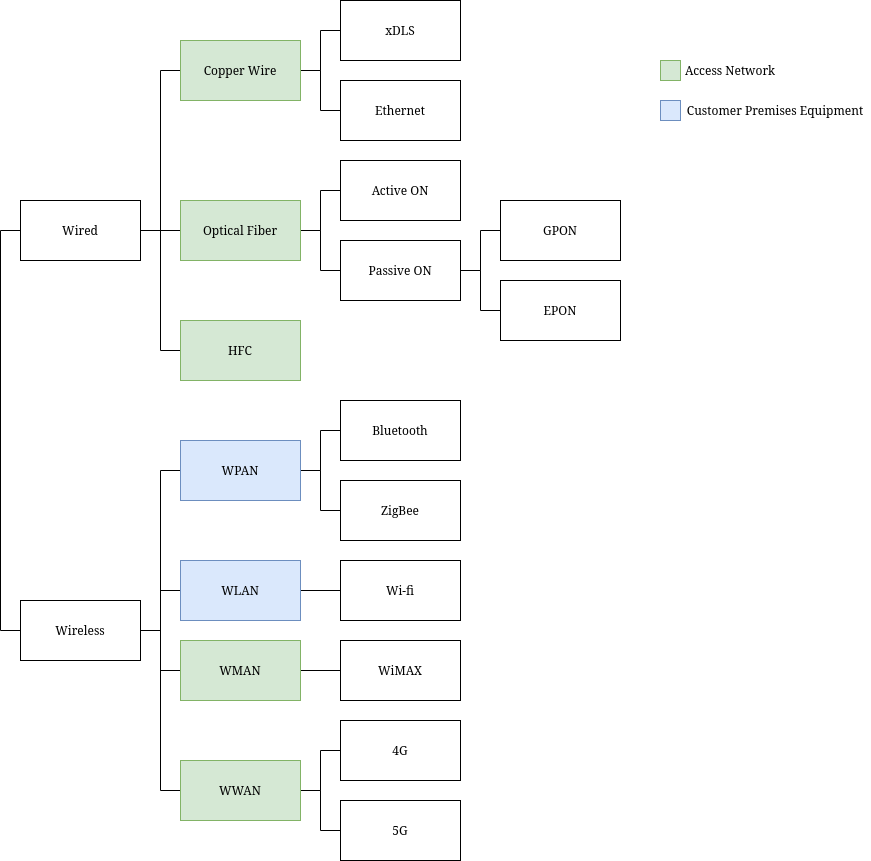
\includegraphics[width=0.8\textwidth]{figs/network_technologies.png}
    \caption[Network technologies used in Access Networks and CPE]{Network technologies used in Access Networks and CPE. In green are the technologies used in the access network and in blue are the technologies used in the CPE. Adapted from \citet{forum:huawei}.}
    \label{figure:network_technologies}
\end{figure}

The first layer and most simple one is the \ac{cpe}. The \ac{cpe} is the equipment that is installed in the end user premises. 
The equipment is usually provided by the \ac{isp} and normally consists of a gateway that acts as a modem and a router.
A modem is used to convert the signal from the \ac{isp} to a signal that can be used by the router. The router is used to connect the end user devices to the internet. The user can connect to the routers either by cable or by wireless technology like Wi-Fi. 

Access networks serve as the connection between the \ac{cpe} and the core network. All users are connected to a central office where traffic is aggregated and then transferred to the core network.
The access network incorporates any technology that establishes the connection between the end user and the \ac{isp} and this technology it is not own by the user. % So a user can connect to the internet by either a modem or a cellular tower but only the cellular tower is part of the access network. 

Traffic in the access network is highly variable. The equipment used in the access network has a power consumption that is largely constant in time and thus load-independent \cite{Vereecken2011}.

\subsubsection{Access Network Wired technologies}

The most popular wired connections are \ac{dsl}, coaxial cable and fiber-optics.

\begin{itemize}

    \item \ac{dsl} provides internet access over existing analog telephone lines. So, existing telephone service providers offer \ac{dsl} service. With this technology, user voice and data traffic go through the analog lines. \ac{dsl} uses high frequencies for data transmission and with the help of \ac{dsl} filter data traffic do not interference with voice traffic.
    There are different DSL types. Currently, \ac{adsl} is the most used \ac{dsl} type in the world. 

    \item \ac{hfc} uses the same coaxial cable that is used for cable television. It uses the \ac{docsis} standard to provide internet access.

    \item Fiber-optic networks use light pulses transmitted through glass or plastic fibers, which produce high bandwidth and transmit speeds. 
    The fibers are also more resistant to interference and signal degradation, making them better suited for sending data over long distances without losing signal quality.
    Fiber optics technology, namely \ac{epon}, have become the most popular choice for wired access network technology. \ac{epon} is a point-to-multipoint network, which means that a single optical fiber is used to serve multiple end users. This is done by using a passive optical splitter, which splits the signal into multiple data streams that are sent to each end user.

\end{itemize}


\subsubsection{Access Network Wireless technologies}

Wireless access networks use radio waves to provide fixed or mobile access services for users. 
According to coverage range classification, the broadband wireless access technology are generally divided into different categories, such as: \ac{wpan}, \ac{wlan}, \ac{wman}, and \ac{wwan}. However, only technologies in the \ac{wman} and \ac{wwan} fall into the umbrella of what we refer to as the access network.

The area coverage of \ac{wman} is in the order of kilometers and there are two prominent technologies to establish internet access, \ac{lmds} and \ac{wimax}.

\begin{itemize}

    \item \ac{lmds} is a multipoint communication system. It is used to provided network connectivity to buildings. These are great technologies for last mile connectivity, because they are more cost-effective than wired technologies and can be deployed faster than fiber \cite{forum:imda}.

    \item \ac{wimax}  is based on IEEE 802.16. It provides fixed, mobile or portable wireless connections, with high speeds that can reach up to 70 \ac{mbps} \cite{forum:ctrfantennasinc}.

\end{itemize}

The \ac{wwan} has a bigger range that the \ac{wman} and is used to provide internet access to mobile devices.
\ac{wwan} uses telecommunication cellular network technologies such as 2G, 3G, 4G LTE, and 5G to transfer data.


\subsection{Core Network}

Core networks consist of several core nodes that are interconnected by \ac{wdm} optical fiber links.

\ac{wdm} is a fiber-optic transmission technique that enables the use of multiple light wavelengths (or colors) to send data over the same medium. Two or more colors of light can travel on one fiber, and several signals can be transmitted in an optical waveguide at differing wavelengths or frequencies on the optical spectrum. 

Each core node is composed by a mix of several layers of technologies stacked on top of each other. Typically, it is composed of a \ac{ip} layer, a \ac{wdm} layer and a \ac{oxc} layer.

From a broad perspective, core nodes operate on an optical-electrical-optical basis. This implies that any optical traffic undergoes conversion into the electronic domain and is then processed by the node, regardless of whether the traffic is terminated at that node. Typically, a node comprises several \ac{wdm} transmit and receive cards, commonly known as transponders or transceivers, which are linked to an \ac{ip} router. The \ac{ip} router, in turn, can establish connections with various access routers.

\section{Datacenters}

Datacenters are facilities that house numerous computing and storage devices. They provide users with the opportunity to host their applications as well as store data. Their use is widespread, and their energy impact is substantial, as they are responsible for  1-1.3\% of the global energy consumption \cite{IEA}.

Datacenters are composed of electronic equipment for communication, data processing and storage. The quantity and type of equipment depends on the type of datacenter. Usually, we can distinguish the type of datacenter by its size and processing power. \citet{Shehabi2016} classifies datacenters in the following categories:

\begin{itemize}
    \item Closet;
    \item Room;
    \item Localized;
    \item Midtier;
    \item High-end;
    \item Hyperscale.
\end{itemize}

The main contributors for the energy consumption of datacenters are the servers, the network and the storage devices. Each type of datacenter has a different efficiency in the use of energy. The efficiency of a datacenter is measured by the \ac{pue}, which is the ratio between the total energy consumption of the facility and the energy consumption of the \ac{it} equipment. The closer it is to one, the better the efficiency of the datacenter.

\subsection{Datacenter Servers}

Datacenter servers are the main component of the datacenter. The servers are computers with the resources capable of executing applications and processing data.

As the main component of the datacenter, they are also the main contributor for the energy consumption of it. According to \citet{Cheung2018} and \citet{Dayarathna2016} the servers account for around 70\% of the energy consumption of the datacenter, ignoring cooling and other non \ac{it} factors.


\subsection{Datacenter Storage}

Storage in datacenters is composed of several \acp{hdd} and \acp{ssd} that are connected to the servers. The storage configuration can be divided in three categories: \ac{das}, \ac{nas} and \ac{san} \cite{Storage101}.

\subsubsection{\acl{das}}

As the name suggests, the storage devices connect directly to the server without any networking. \ac{das} can connect either internally or externally, as a single drive or an array of \ac{raid}. 

Of the three types, \ac{das} is the easier and cheapest option. However, it is also the least scalable and the least flexible, because the server has a limited number of ports and expansion slots.

\subsubsection{\acl{nas}}

\ac{nas} is a centralized file-level storage system, that is connected to the server via the network. \ac{nas} is composed of a storage device with an \ac{os} that is optimized for file storage and sharing.

It includes built-in fault tolerance, management capabilities, and security protections, and it can support features such as replication and data deduplication.

\subsubsection{\acl{san}}

\ac{san} is a decentralized block-level storage system, that is connected to the server via the network. It presents a pool of block-level storage to the server, which the server can then format and partition as it sees fit.

It is composed of storage arrays (\acp{raid}), servers for managing data access, storage management software, \acp{hba}, and any physical components that make up the network's infrastructure.

\subsection{Datacenter Network}

Typically, datacenter networks are composed of switches, routers and other hardware components that provide the connectivity and security to run applications and process data on the servers. 
According to \citet{Cheung2018} and \citet{Dayarathna2016} the network accounts for around 10\% of the energy consumption of the datacenter. 

Today there are three main topologies that datacenters can follow, but larger datacenters can use two or all three of them. Each topology has its own advantages and disadvantages, and the choice of topology depends on the type of datacenter and the type of applications that it will be hosted \cite{commScope}.

\subsubsection{Centralized}

This model is more used by smaller datacenters. There are separated environments for the server and storage, with dedicated  cables that connect the storage server cabinets to the storage.  

\subsubsection{\ac{eor}}

This topology consists in distributing network resources, as seen in Figure \ref{figure:eor_topology}. The servers are placed in rows and the network resources are placed at the end of each row. This solution is recommended by the  ANSI/TIA-942 Data Center Standards \cite{ANSI/TIA-942} and is very scalable, repeatable, and predictable.

\begin{figure}[h]
    \centering
    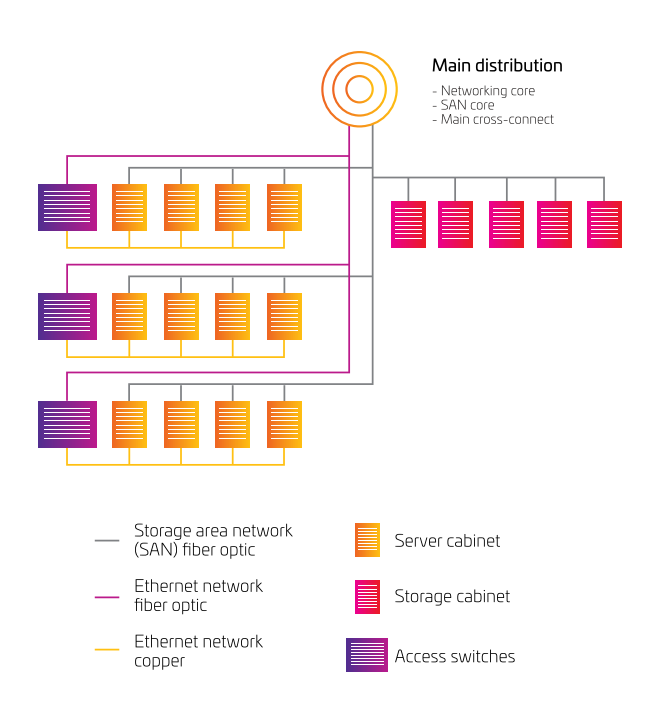
\includegraphics[width=0.8\textwidth]{figs/eor_topology.png}
    \caption[End of Row topology.] {End of Row topology, adapted from \citet{commScope}.}
    \label{figure:eor_topology}
\end{figure}

\subsubsection{\ac{tor}} 

Top of the rack consists on two or more switches on top of each server cabinet, as shown in Figure \ref{figure:tor_topology}. It is cost-effective, because it reduces the number of copper cables between racks. The rack is linked to the data center network by an Ethernet switch, often through a fiber cable. This fiber cable is a direct link from the common aggregation area to the rack.
In the \ac{tor} approach, every rack in the data center network is a separate entity that eases its management. Any change, upgrade, or malfunction in the rack usually affects that rack only.

\begin{figure}[h]
    \centering
    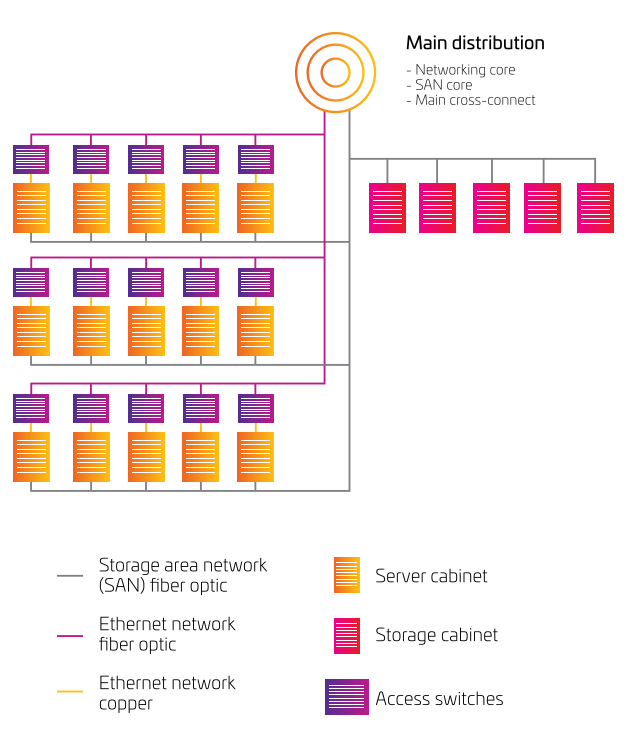
\includegraphics[width=0.8\textwidth]{figs/tor_topology.png}
    \caption[Top of Rack topology.] {Top of Rack topology, adapted from \citet{commScope}.}
    \label{figure:tor_topology}
\end{figure}

\section{Data compression algorithms}

Compression algorithms are used to reduce the size of a file or data stream. They have been used in applications where the cost of storage or transmission is high.

With the increase of the use of the internet and the increase of the amount of data that are stored and transmitted, compression algorithms have become a standard in the \ac{ict} sector.

\subsubsection{Lossless compression}

Lossless algorithms usually exploit the redundancy present in data to reduce the size without losing any information. Among the lossless algorithms, the Lemple-Ziv (LZ) family of algorithms are the most popular. One popular image format that uses lossless compression is the \ac{png} format. The \ac{png} format uses the DEFLATE algorithm \cite{rfc1951}, which is a combination of LZ77 and Huffman coding.

\subsubsection{Lossy compression}

Lossy compression algorithms are used when the loss of information is acceptable. They are usually used in multimedia applications, where the loss of information is not noticeable, or is tolerable by the end user.

\subsection{Compression algorithms overview}
\label{section:compression_algorithms_overview}

Compression algorithms can be divided in two categories based on the type of data that they are used to compressing. General purpose algorithms can be used to compress any type of data. Specific algorithms, on the other hand, are developed to compress a specific type of data, like images, audio or even genetic data, and are usually more efficient in their data type than general purpose algorithms.

There exists several compression algorithms available, their characteristics are summarized in Table \ref{table:compression_algorithms}.

\begin{table}
\caption{Compression algorithms and their characteristics.}
\label{table:compression_algorithms}
\begin{center}
    \begin{tabular}{|| c | c | c ||}
        \hline
        Name & Data type & Reference \\
        \hline
        Gzip        & Any & \citet{rfc1952}\\ \hline
        Zstandard   & Any & \citet{rfc8878}\\ \hline
        Bzip2       & Any & \citet{bzip2}\\ \hline
        LZMA        & Any & \citet{lzma}\\ \hline
        Cmix        & Any & \citet{cmix}\\ \hline
        PAQ1        & Any & \citet{Mahoney2002}\\ \hline
        NNCP        & Any & \citet{NNCP}\\ \hline
        MFCompress  & FASTA, multi-FASTA & \citet{Pinho2014}\\ \hline
        Jarvis3     & FASTA, FASTQ & \citet{jarvis3}\\ \hline
        Naf         & FASTA, FASTQ & \citet{Kryukov2019}\\ \hline
        Leon        & FASTA, FASTQ & \citet{Benoit2015}\\ \hline
        Agc         & FASTA & \citet{Deorowicz2023}\\ \hline
        Fqzcomp     & FASTQ & \citet{fqzcomp}\\ \hline
        Quip        & SAM/BAM & \citet{Jones2012}\\ \hline
    \end{tabular}
\end{center}
\end{table}

\subsubsection{General purpose algorithms}

As stated above, compression algorithms can be divided into two categories, general purpose and specific algorithms. In terms of general purpose algorithms, we have the most popular algorithms, Zstandard, Gzip, Bzip2 and LZMA \cite{GeekyHumans}.

Zstandard and Gzip are both lossless compression algorithms based on the DEFLATE algorithm, which uses a combination of both LZ77 and Huffman coding. Zstandard is the most recent algorithm and was developed by Facebook, offering a much faster compression and decompression than its predecessors. Gzip was created as an alternative to the compress program in Unix systems, because of the Unisys and IBM patents covering the LZW algorithm.

Bzip2 is a lossless compression algorithm based on the Burrows-Wheeler transform. It is more efficient than DEFLATE but is also slower. Even though it can be used in any type of data it is most efficient in text based data. The algorithm is composed of several compression techniques such as \ac{rle}, Burrows-Wheeler transform, move-to-front transform and Huffman coding.

LZMA is a lossless compression algorithm based on the Lempel-Ziv-Markov chain algorithm. It is used by the 7zip file archiver and the xz file format.

Cmix and PAQ are both context mixing compression algorithms. They use more than one model to predict the next symbol in a sequence, it usually results in a more accurate prediction than using only one model. Cmix uses several machine learning models, while PAQ1, a version of the PAQ, uses a weighted average of 5 bit-level predictors.

NNCP also uses machine learning models, in this case it uses pure neural network models based on the \ac{lstm} and Transform model.

\subsubsection{Specific algorithms}

In terms of specific algorithms, we focus on algorithms that compress genome sequences. These algorithms compress files that are in the FASTA, FASTQ and \ac{sam}/\ac{bam} formats.

\subsubsection{Genome sequence formats}

Genome sequencing is a process that determines the order of the nucleotides in a genome, it turns sequences of genomes into data that can be stored and analyzed. The genome sequence is usually stored in a file, which can be in several formats. The most common formats are FASTQ, FASTA, \ac{sam}/\ac{bam} and \ac{vcf}.

FASTQ is a text-based format that stores the biological sequence and its corresponding quality scores. Each entry of the file is composed of 4 lines. The first line is the sequence identifier, the second line is the genetic sequence (the nucleotide bases A, C, T, G and N), the third line is a separator, lastly the fourth line is the quality score of each base.

FASTA is also a text-based format that stores the biological sequence. However, it only stores the headers and nucleotide bases sequenced, which makes it more compact than FASTQ.

\ac{sam}/\ac{bam} are the text and binary versions of the same format. They are used to store the alignment of the sequenced reads to a reference genome. The file is composed of a header and a body. The header contains information about the reference genome and the body contains the alignment of the reads. They reduce the space needed to store a genetic sequence however they are dependent on a reference genome.

Lastly \ac{vcf} is the standard file format for storing variation data. It is used by large scale variant mapping projects such as IGSR. It is also the standard output of variant calling software such as GATK and the standard input for variant analysis tools such as the VEP or for variation archives like EVA.
VCF is a preferred format because it is unambiguous, scalable and flexible, allowing extra information to be added to the info field. Many millions of variants can be stored in a single VCF file. 

MFCompress was designed and implemented in \ac{ieeta}. It is a tool for compressing FASTA and multi-FASTA files, achieving compression gains of almost 50\%. The algorithm bases on probabilistic models that comply with the Markov property, i.e. that estimate the probability of the next symbol of the information source using the $k>0$ immediate past symbols (order-k context) to select the probability distribution. 

Jarvis3, NAF and Leon, are tools that compress FASTA and FASTQ files, but all focus on different techniques. Jarvis3 uses neural network models, while NAF is based on the Zstandard algorithm. Leon uses probabilistic models based on "De Bruijin Graph", it has the advantage of not needing to have a reference genome for the execution of the algorithm.

Agc uses a reference genome to compress FASTA files, and in small sequences it uses Zstandard.

Fqzcomp compresses FASTQ files and uses ZPAQ, an algorithm of the PAQ family, to achieve higher levels of compression.

Lastly Quip compresses FASTQ and \ac{sam}/\ac{bam} files using reference-based arithmetic encoding.


% estado da arte de algoritmos especificos
% algoritmos usados pelo ENA european nucleotide archive e SRA
% zstandard gzip bzip2 lzma 
% especificos fqzcomp quip leon 
% dsrc2 

% tipos de dados:
% fastq fasta sum/bam vcf

% seqSqueeze

% mfcompress
% jarvis3
% naf agc

% cmix
% paq1-9
% nncp




\chapter{Related Works}
\label{chapter:related_works}

\begin{introduction}
    Many authors have tackled the problem of estimating the energy consumption of parts of the \ac{ict}. However, very few have tried to estimate the energy consumption of the \ac{ict} as a whole. To make sure that the most appropriate models are used in this thesis, a review of the most recent studies was made. This review includes the criteria for selecting these models, a description on how the models work and the system boundary they act upon, and the pitfalls and assumptions of each model.
\end{introduction}

\section{Systematic review methodology}

The search methodology focused on studies that analyze energy or carbon consumption of parts of the \ac{ict} sector, such as datacenters. The search was based primarily on English language publications, using bibliographic databases such as IEEE Xplore Digital Library (\textbf{link}), ResearchGate (\textbf{link}). ACM Digital Library (\textbf{link}) and Google Scholar (\textbf{link}). Also, to complement the search we used ConnectedPapers (\textbf{link}), a tool that uses the references of a paper to create a graph of papers similar to the reference.

The search was based on primarily done by using a keyword related to the specific area of the \ac{ict} sector in study followed by a keyword related to energy consumption. For example a search for datacenters would be done by using the keywords \textit{"datacenter"} and \textit{"power consumption"}. The search filtered articles to include only those above January 2000. 
From the results gathered papers that showed bottom-up models were privileged over top-down models. 

\section{Energy consumption studies}

In this section, we will present the most relevant studies gathered by the methodology described in the previous section. Each study tackles a different subsystem, however, their boundary delimitation can overlap with others, so we will frame the boundaries of the studies into the system boundaries that we have defined in \ref{section:system_boundaries}.

The methodology used by each study is different. We separate the studies into those who use modeling, direct measurement, and those who use a combination of both.

\subsection{Modeling}

This approach consists in specifying equations based on parameters like energy consumption to describe the subsystem in study. The parameters can be obtained by using empirical data or by making informed assumptions of the system in question. 

\citet{Coroama2015} uses both approaches to estimate the energy consumption of the \ac{cpe} and access network subsystems. They developed a formula for estimating the energy intensity of these two subsystems. The formula, (\ref{formula:coroama_cpe_an}), builds on their previous analysis of multimedia servers \citet{Schien2013} 

\begin{equation}
\label{formula:coroama_cpe_an}
    I_{CPE,AN} = \frac{t_{on}}{t_{use}} \frac{P_{CPE}}{N_{CPE}} + \frac{P_{AN}}{N_{AN}} PUE_{AN}
\end{equation}

\begin{itemize}
    \item $I_{CPE,AN}$: Intensity of both \ac{cpe} and \ac{an}.
    \item $\frac{t_{on}}{t_{use}}$: Ratio of time that the device is actively working. 
    \item $P_{CPE}$: Power of all \ac{cpe} devices.
    \item $N_{CPE}$: Number of Users connected to the \ac{cpe}.
    \item $P_{AN}$: Power of all \ac{an} devices.
    \item $N_{AN}$: Number of users (subscribers) connected to the \ac{an}.
    \item $PUE_{AN}$: \ac{pue} of the \ac{an}.
\end{itemize}

$\frac{P_{AN}}{N_{AN}}$ gives the energy intensity of the \ac{an} per subscriber, the technology they evaluate is \ac{adsl2} which has a power consumption of \SI{2}{\watt} per subscriber \citet{Schien2013}. As for the $PUE$ they assume a value of 2. 
$\frac{P_{CPE}}{N_{CPE}}$ gives the energy intensity of the \ac{cpe} per subscriber. The study assumes that each household has 2 \ac{cpe} devices, a modem and a router, and arrives at a value of \SI{8}{\watt} per subscriber when accounting for legacy equipment. 
The ratio of time that the device is actively working is estimated to be 6 according to the findings in \citet{Nissen2007}.
The study then concludes that the energy intensity for this subsystem is \SI{52}{\watt} per subscriber.

\citet{Schien2015} developed a model for the subsystem of core network. The study created a model to estimate the energy consumption of data traffic in the core network, that is the cost per \ac{gigabyte} of data transmitted. 
The model only considers the devices that will carry the connection data between the user and the server. Because not all energy spent by each device is directly related to a request, the energy intensity is the ratio between the energy spent by the device and the data throughput.   



\subsection{Direct measurement}



% \subsection{Structure of the Internet}

% The internet is a network of networks, an infrastructure comprised of billions of computers, 
% using protocols,\ac{tcp}/\ac{ip} to communicate.

% It has always been a challenge to estimate the energy consumption of the internet, because of the complexe structure of the network. Nonetheless, several studies have been made to estimate the energy consumption. However, the results of the studies can go from 136 \ac{kilowatt-hour}/\ac{gigabyte}
% \citet{Koomey2003} down to 0.0064 \ac{kilowatt-hour}/\ac{gigabyte} \citet{Baliga2011}.

% As \citet{Coroama2015} and later \citet{Aslan2018} point out, the difference in results is due to the year that the study is made and the scope of the study. 
% The year is important because the energy efficiency of the equipment has been improving over the years. 
% The scope or system boundary is important because the studies can map different layers of the network.

% The internet is usually divided in layers as seen in the figure \ref{fig:layers}. 
% Each layer handles different amount on traffic so has different energy needs.
% The structure of the layers is discussed in the following sections.  

% \subsubsection{\acl{cpe} and Access network}

% In telecomunications, \ac{cpe} is the equipment that is installed in the end user premises that connects to the provider network. This usually means wifi routers and modems that connect to their \ac{isp} through a feeder network. The \ac{isp} bundles the data transmited by several end users in multiplexers, which for the case of \ac{isp} that use \ac{dsl} connectivety they are \ac{dslam}. The multiplexers and the cables that connect them to the \ac{cpe} are what constitute the access network.

% \subsubsection{Core network}

% Core network or IP core network is the network that interconnects several \ac{isp} with each other, forming the regional and global networks.
% The network consists of routers, switches, and other network infrastructure that directs data packets across the network. These devices use routing algorithms and protocols to determine the best path for data to travel based on factors like network congestion and available bandwidth.

% \subsection{Datacenters}

% Datacenters are facilities that house computer systems and associated components. They are a larges contributer to energy consumption in the internet, consuming a total of 205 \ac{terawatt-hour} in 2020, or 1\% of global eletric power \citet{IEA2020}. 
\chapter{Energy Model}
\label{chapter:energy_model}

\begin{introduction}
    As seen in the previous chapter, no uniform model exists for the energy consumption of the \ac{ict}. This is due to the complexity of the \ac{ict} and the different components that can be used.

    This chapter explains how the aggregated model was constructed as well as how the compression algorithms impact the energy calculation.
\end{introduction}


\section{Description of the work}

    The aggregated model needs to have a wide system boundary and encapsulate each component of the \ac{ict}. Based on the work of chapter \ref{chapter:related_works}, three studies were selected to make up the model. These studies were chosen because they cover a wide system boundary with little overlap, as well as having a complete and easily modifiable formula.
    
    \begin{table}
        \caption{Selected energy models and their system boundaries.}
        \label{table:selected_energy_models}
        \begin{center}
            \begin{tabular}{|| c | c | c | c | c | c ||}
                \hline
                \multirow{2}{*}{Study} & \multirow{2}{*}{Year of data} & \multicolumn{4}{c||}{System Boundary} \\ \cline{3-6}
                & & \ac{cpe} & \ac{an} & Core Network & Datacenter \\
                \hline
                \citet{Coroama2015}     & 2014 & \checkmark & \checkmark &  &   \\ \hline
                \citet{Schien2015}      & 2014 &  &  & \checkmark &   \\ \hline
                \citet{Taal2014}        & 2013 &  &  & \checkmark & \checkmark  \\ \hline
            \end{tabular}
        \end{center}
    \end{table}

    Table \ref{table:selected_energy_models} shows the studies that were selected and the components they cover. Only the Datacenter part of \citet{Taal2014} was considered as the other part was already covered by the former studies. 
    
    With the models for each component, the next step was determine how the compression algorithms would impact the energy consumption.
    The model represents three stages:
    \begin{itemize}
        \item The Upload stage, where data is uploaded into the datacenters and where compression can be applied.
        \item The Storage stage, where the data is stored in the datacenters.
        \item The Download stage, where the data is downloaded from the datacenters and the process of decompression is applied on the user devices.
    \end{itemize} 

    Figure \ref{figure:energy_model_stages}
    shows which components and subcomponents each stage interacts with, the arrows show the flow of data between the components. 
    As we can see both the Upload and Download stages interact with the whole system while the Storage stage only interacts with the Datacenter's storage subcomponent. Joining the three stages together, we have the complete  model.
    
\section{Upload Stage}

\subsection{Energy Model}

    As seen in the previous section, the Upload stage interacts with the user, the network and the Datacenter components. So we can describe this stage as the sum of the energy consumption of the user, network and Datacenter components,

    \begin{equation}
        \label{formula:upload_stage}
        E_{upload}(D_{in}) = E_{user}(D_{in}) + E_{network}(D_{in}) + E_{datacenter}(D_{in}),
    \end{equation}

    \noindent with $D_{in}$ being the data that is uploaded, or as we refer in this paper, the input data. 

    Now we need to choose the most adequate model for calculating the energy consumption of each component.

    For the user component, we choose to define its energy consumption based on the time it takes for the task to be completed, in this case, the task is the upload of data, and the energy intensity of the devices, similar to how \citet{Coroama2015} defined for the \ac{cpe}. So we express the energy consumption as the following:

    \begin{equation}
        \label{formula:upload_user_energy}
        E_{user}(D_{in}) = \frac{D_{in}}{R_{upload}} \cdot P_{user\_device},
    \end{equation}

    \noindent where $R_{upload}$ is the upload rate of the user device, in MB/s, which by dividing $D_{in}$ with it, we have an approximate value of the time it takes upload the data, or in other words, the active time. $P_{user\_device}$ is the power consumption of the user device. Multiplying the active time by the power consumption, we have the desired energy consumption of the user component.

    For the network component, we use the formula of energy intensity of \citet{Coroama2015}, \ref{formula:coroama_cpe_an}. As sated in the previous chapter, the energy consumption of \ac{cpe} and \ac{an} are dependent on the time they are active for the workload to complete, not the amount of data. So we have to use the active time calculated in the user component and multiply with the energy intensity of the network component. Resulting in:

    \begin{equation}
        \label{formula:upload_network_energy}
        E_{network}(D_{in}) = \frac{D_{in}}{R_{upload}} \cdot \Bigg( \frac{t_{on}}{t_{use}} \cdot \frac{P_{CPE}}{N_{CPE}} + \frac{P_{AN}}{N_{AN}} \cdot PUE_{AN} \Bigg).
    \end{equation}
    
    As for the core network part, we use the formula of \citet{Schien2015}, shown in \ref{formula:schien_core_metro}, this component however is not time based, but purely data based, so there is no need to alter the formula.

    Lastly for the Datacenter component, we use the formula of \citet{Taal2014} that covers the server write operation, \ref{formula:tall_datacenter_write}. However, there was the need to make some changes to the equation to fit with our model.

    First, there is a correction to the equation for calculating the number of disks (\ref{formula:tall_datacenter_ndisks}) needed to store the data, as the size of the array doesn't influence the number of disks needed.
    The new formula is the following:
    \begin{equation}
        \label{formula:storage_ndisks}
        N_d(D_{in}) = 2 \cdot \bigg \lceil \frac{D_{in}}{S_{disk}} \bigg \rceil,
    \end{equation} 
    \noindent with:
    \begin{itemize}
        \item $S_{disk}$ is the size of the disk.
    \end{itemize}

    Another change is that we removed the conversion of Gbps to GBph, that was used in the original formula, as the data is already in the correct format, and we removed the utilization factor ($U$) as it is not needed for the model.

    Finally, we changed the name of the term capacity to bandwidth, as it is more fitting for the context of the formula, and unraveled the terms to make it easier for when we apply compression later on.

    The final formula is the following:

    \begin{equation}
    \label{formula:upload_server_write}
    \begin{split}
        E_{write}(D_{in}) = & \Bigg( \frac{D_{in}}{B_{server}} \cdot P_{server} + \\ & \frac{D_{in}}{B_{sw}} \cdot P_{sw} + \\ & \frac{D_{in}}{B_{disk}} \cdot P_{disk} \cdot N_d(D_{in}) \Bigg) \cdot PUE,
    \end{split}
    \end{equation}

    \noindent where:
    \begin{itemize}
        \item $B_{server}$ is the capacity of the server.
        \item $B_{sw}$ is the capacity of the switch.
        \item $B_{disk}$ is the capacity of the disk.
        \item $P_{server}$ is the power consumption of the server.
        \item $P_{sw}$ is the power consumption of the switch.
        \item $P_{disk}$ is the power consumption of the disk.
        \item $N_d(D_{in})$ is the number of disks needed to store the data.
        \item $PUE$ is the Power Usage Effectiveness of the datacenter.
    \end{itemize}

\subsection{Energy Model while using compression}

    The use of compression algorithms will affect how the model is calculated, because it will introduce two variables, the compression rate $c_{rate}$, which is the rate that data will be reduced by when applying compression, and the additional time it takes to compress the data, the compression time cost ($c_{t\_cost}$).

    The input data ($D_{in}$) still refers to the size of the original data without applying compression.

    We defined that data is compressed server-side, so only the formula of the Datacenter component will be affected by the compression time cost. The new formula is the following:
    
    \begin{equation}
    \label{formula:upload_server_write_compressed}
    \begin{split}
        E_{write}(D_{in}) = & \Bigg( \bigg(\frac{D_{in}}{B_{server}} \cdot D_{in} \cdot c_{t\_cost} \bigg) \cdot P_{server} + \\ & \frac{D_{comp}(D_{in})}{B_{sw}} \cdot P_{sw} + \\ & \frac{D_{comp}(D_{in})}{B_{disk}} \cdot P_{disk} \cdot N_d(D_{comp}(D_{in})) \Bigg) \cdot PUE,
    \end{split}
    \end{equation}

    \noindent where:
    \begin{itemize}
        \item $D_{comp}(D_{in})$ is the size of the compressed data, $D_{comp}(D_{in}) = \frac{D_{in}}{c_{rate}}$.
        \item $c_{t\_cost}$ is the time cost of compressing the data.
        \item $B_{server}$ is the capacity of the server.
        \item $B_{sw}$ is the capacity of the software.
        \item $B_{disk}$ is the capacity of the disk.
        \item $P_{server}$ is the power consumption of the server.
        \item $P_{sw}$ is the power consumption of the software.
        \item $P_{disk}$ is the power consumption of the disk.
        \item $N_d(D_{in})$ is the number of disks needed to store the data.
        \item $PUE$ is the Power Usage Effectiveness of the datacenter.
    \end{itemize}

    As we can see, different parts of the datacenter will deal with different amounts of data, because the server has to process the original data as well as deal with compression, so an additional process time $c_{{t\_cost}}$ is factored.
    The other subcomponents will receive the already compressed data, which will lower their overall energy consumption.

    As for the rest of the model, as their stages happen before the compression, they will not be affected by it, so their formulas remain the same, as the data is still in the original form.

\section{Storage Stage}

\subsection{Energy Model}
    The storage stage is the smallest of the three stages, as it only interacts with the Datacenter's storage subcomponent. The energy consumption of this stage the formula of \citet{Taal2014} that covers the server store operation, equation \ref{formula:tall_datacenter_store}. The equation that the study used was mostly adequate for our model, and the only change needed to be made was removing the utilization factor ($U$) like we did in the upload stage equation.

\subsection{Energy Model while using compression}

    The use of compression will only affect the size of the input data, so the only change in the formula is applying the compression rate to the input data.
    Resulting in the final formula:
    \begin{equation}
        \label{formula:storage_stage}
        E_{storage}(D_{in}) = PUE \cdot N_d(D_{comp}(D_{in})) \cdot P_{disk} \cdot RT,
    \end{equation}

    \noindent with:
    \begin{itemize}
        \item $D_{comp}(D_{in})$ is the size of the compressed data, $D_{comp}(D_{in}) = \frac{D_{in}}{c_{rate}}$.
        \item $N_d(D_{in})$ is the number of disks needed to store the data.
        \item $P_{disk}$ is the power consumption of the disk.
        \item $RT$ is the retention time of the data.
    \end{itemize}

\section{Download Stage}

\subsection{Energy Model}

    The download stage is like the mirror of the upload stage, as it interacts with the same components, but the flow of data is reversed. So like the former stage, the energy consumption is the sum of the energy consumption of the user, network and Datacenter components.

    \begin{equation}
        \label{formula:download_stage}
        E_{download}(D_{out}) = E_{user}(D_{out}) + E_{network}(D_{out}) + E_{datacenter}(D_{out}),
    \end{equation}

    \noindent with $D_{out}$ being the size of all data being downloaded.

    The active time is now based on the download rate ($R_{download}$) and the amount of data downloaded ($D_{out}$).

    The user component is the same as in the upload stage, \ref{formula:upload_user_energy}, with the upload rate being replaced by the download rate.

    The network component will use the same formula from \ref{formula:coroama_cpe_an} as used in the upload stage, but with the different active time.
    As for the core network part, it remains the same as in the upload stage.

    Lastly for the Datacenter component, we use the formula of \citet{Taal2014} that covers the server read operation, \ref{formula:tall_datacenter_read}. Like with the upload stage, we applied the same changes, that is, removed the utilization factor ($U$) and conversion from Gbps to BGph, and changed the term capacity to bandwidth. The final formula became the following: 

    \begin{equation}
    \label{formula:download_server_read}
    \begin{split}
        E_{read}(D_{out}) = PUE \cdot D_{out} \cdot \Bigg( \frac{P_{server}}{B_{server}} + \frac{P_{sw}}{B_{sw}}\Bigg),
    \end{split}
    \end{equation}

    \noindent where:
    \begin{itemize}
        \item $B_{server}$ is the capacity of the server.
        \item $B_{sw}$ is the capacity of the switch.
        \item $P_{server}$ is the power consumption of the server.
        \item $P_{sw}$ is the power consumption of the switch.
        \item $PUE$ is the Power Usage Effectiveness of the datacenter.
    \end{itemize}

\subsection{Energy Model while using compression}

    This stage deals with the data in the compressed form and with the task of decompressing it, so a new variable is introduced, the decompression time cost $d_{t\_cost}$.
    
    The data is decompressed on the user device, so for the components before the user device, the data is still in the compressed form, so the datacenter and network equations have to use the compressed data size.

    As for the user component we need to add the decompression step, which is similar to the compression step used in the former stage. The new formula is the following:

    \begin{equation}
        \label{formula:download_user_energy_compressed}
        E_{user}(D_{out}) = \bigg( \frac{D_{comp}(D_{out})}{R_{download}} + D_{comp}(D_{out}) \cdot d_{t\_cost} \bigg) \cdot P_{user\_device},
    \end{equation}

    \noindent where:
    \begin{itemize}
        \item $D_{comp}(D_{out})$ is the size of the compressed data, $D_{comp}(D_{in}) = \frac{D_{in}}{c_{rate}}$.
        \item $R_{download}$ is the download rate of the user device.
        \item $d_{t\_cost}$ is the time cost of decompressing the data.
        \item $P_{user\_device}$ is the power consumption of the user device.
    \end{itemize}


\section{Model Evaluation}

    To evaluate the accuracy of the model, we need to compare the results of the model with real-world data. Although the studies where the formulas were taken from already performed this step, further testing will only reinforce the model's validity.

    However, acquiring real-world data is difficult due to the lack of public data on the energy consumption of the \ac{ict}, so not every component can be tested. We gathered data from \ac{stic} which will help us validate the Datacenter component of the model. 


\section{Conclusion}








\chapter{Compression Algorithms Benchmarking}
\label{chapter:compression_algorithms_benchmark}


\begin{introduction}
    This chapter presents the benchmarking process and results of various compression algorithms. The benchmarking focuses on measuring the time increase in compression and decompression, as well as the compression ratio. By gathering these metrics, we aim to explore any correlation between the time increase and the number of operations performed by each algorithm.

    The results of the benchmarking process provide insights into the performance of the compression algorithms and their suitability for different scenarios. These findings contribute to the understanding of the compression algorithms, enabling us to determine the values to be used for parameters in the energy model. The parameters we aim to determine are the compression ratio ($c_{ration}$), the added compression time increase ($c_{t\_cost}$) and the added decompression time increase ($d_{t\_cost}$).
\end{introduction}

\section{Description of the work}
        The aspects of the compression algorithms that are needed to benchmark are the time increase in compression and decompression and the compression ratio. To gather this data we used the \texttt{perf} profiler to measure the time elapsed, the number of cycles and the number of instructions executed during the compression and decompression of the files. These metrics were gathered to see if there existed any correlation between the time increase and the number of operations each algorithm performed. 
        
        The compression ratio was calculated by dividing the size of the original file by the size of the compressed file. 

\section{Methodology}

    The benchmarking process was done by compressing and decompressing a set of files with different sizes and types. There were three types of files considered:
    \begin{itemize}
        \item Text files, which where gathered from the Project Gutenberg website \url{https://www.gutenberg.org/}.
        Several books were concatenated to create files of approximately 1, 10, 100 and 1000 Megabytes.
        \item Random text files, these are randomly generated text files using the \texttt{/dev/urandom} file, which is a file that generates random data. The sizes of these files are the same as the text files.
        \item Genome sequence files, which were gathered from the NCBI website \url{https://www.ncbi.nlm.nih.gov/}. These sequences are either in the FASTA or FASTQ formats.
    \end{itemize}
    
    The algorithms mentioned in the section \ref{section:compression_algorithms_overview} were used, except for the \texttt{cmix} algorithm due to its large system requirements not making it possible to run on a 16-GB RAM machine. We divided the algorithms into two categories, general purpose and specific. The general purpose algorithms were tested on the text and random text files, while the specific algorithms were tested on the genome sequence files. The \texttt{gzip} algorithm was tested on all files as a way to compare the performance of the specific algorithms.

    % Dizer o porque q se escolheu o gzip para testar todos?

    Each algorithm has a wide set of parameters and tweaks that improve its performance in different scenarios. To make a fair comparison, it was decided to only test the default parameters of each algorithm.

    To account for fluctuations in the system, each algorithm was executed 5 times for each file, and the average of the 5 executions was calculated.

    Due to the large size of files some algorithms would take an unreasonable amount of time to compress and decompress the files, so not every algorithm was tested with every file.
    

\section{Results}

    The results of the benchmarking process are presented in the following sections. We divided the results by the type of algorithm used.

    \subsection{General purpose algorithms}

        As we can see from the following Figures, \ref{fig:text_stats} and \ref{fig:random_text_stats}, independently of the algorithm, the time elapsed, the number of cycles and the number of instructions executed by the algorithms are proportional to the size of the file. This means that the time increase is linear with the size of the file, which is in accordance with the algorithms the compressors use. 

        \begin{figure}[h]
            \centering
            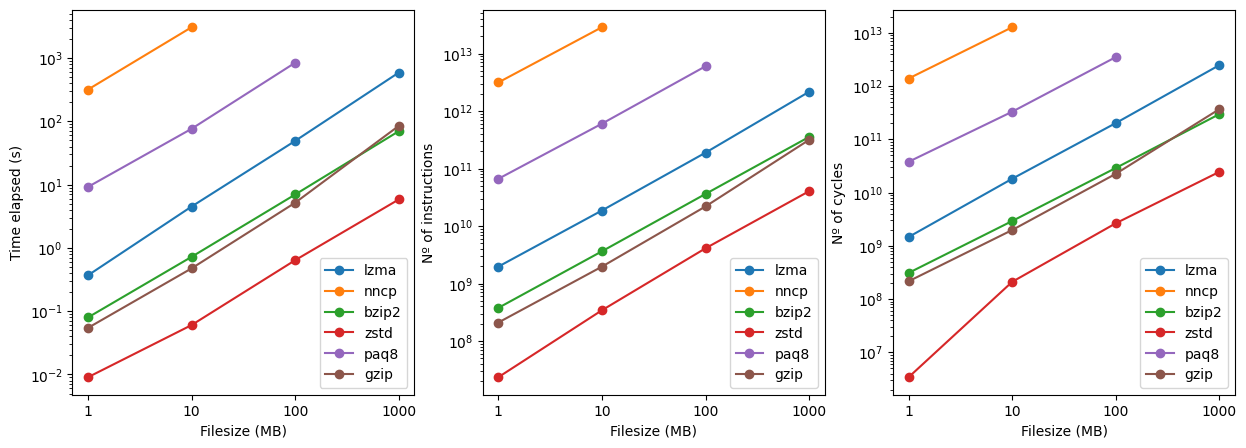
\includegraphics[width=1\textwidth]{figs/text_stats.png}
            \caption[Figure displaying the metrics of the general purpose algorithms when compressing text files.] {Figure displaying the metrics of the general purpose algorithms when compressing text files. The plots display the time elapsed, the number of instructions and the number of cycles executed by the algorithms respectively.}
            \label{fig:text_stats}
        \end{figure}

        \begin{figure}[h]
            \centering
            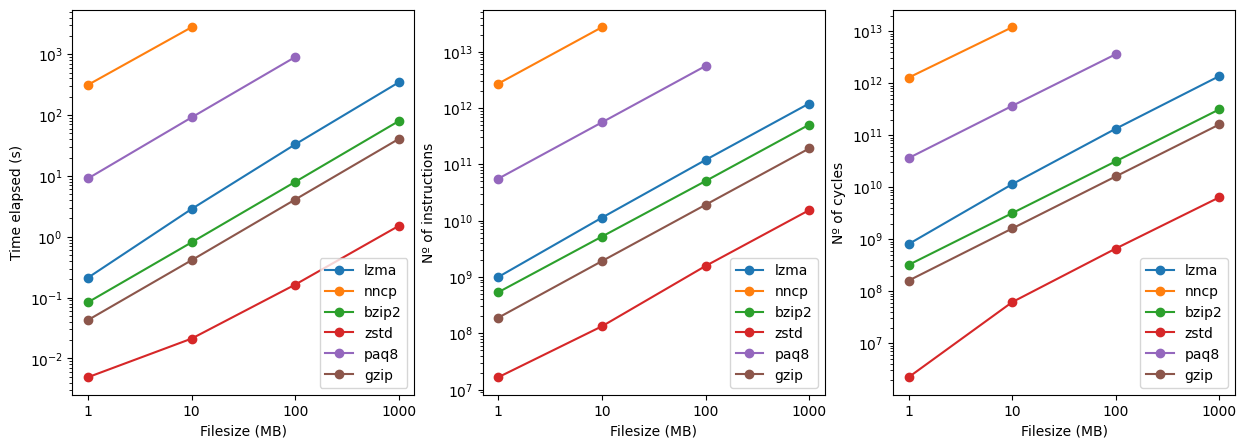
\includegraphics[width=1\textwidth]{figs/random_text_stats.png}
            \caption[Figure displaying the metrics of the general purpose algorithms when compressing random text files.] {Figure displaying the metrics of the general purpose algorithms when compressing random text files. The plots display the time elapsed, the number of instructions and the number of cycles executed by the algorithms respectively.}
            \label{fig:random_text_stats}
        \end{figure}

        Analyzing the metrics we can separate the algorithms into three groups, each separated by at least an order of magnitude in the time metrics.
        The first group comprises solely of \texttt{zstandard}, which proved to be the fastest of the algorithms in all metrics. The second group is composed of \texttt{gzip}, \texttt{bzip2} and \texttt{lzma}, which are the second, third and fourth fastest algorithms, respectively. The third group is composed of the more complex algorithms, such as \texttt{paq8} and \texttt{nncp}, which are the slowest in all metrics. This is expected, as the more complex algorithms need to perform more operations to compress the files.
        
        Changing the type of the file didn't have any significant impact on the time metrics of the algorithms, so time performance isn't related to the data type of the file.

        Observing the compressed size of the files generated by the algorithms, presented in Figures \ref{fig:random_text_comp_size} and \ref{fig:text_comp_size}, and their respectively compression rations, shown in Figures \ref{fig:random_text_comp_ratio} and \ref{fig:text_comp_ratio}, we can see some interesting results. 

        \begin{figure}
            \centering
            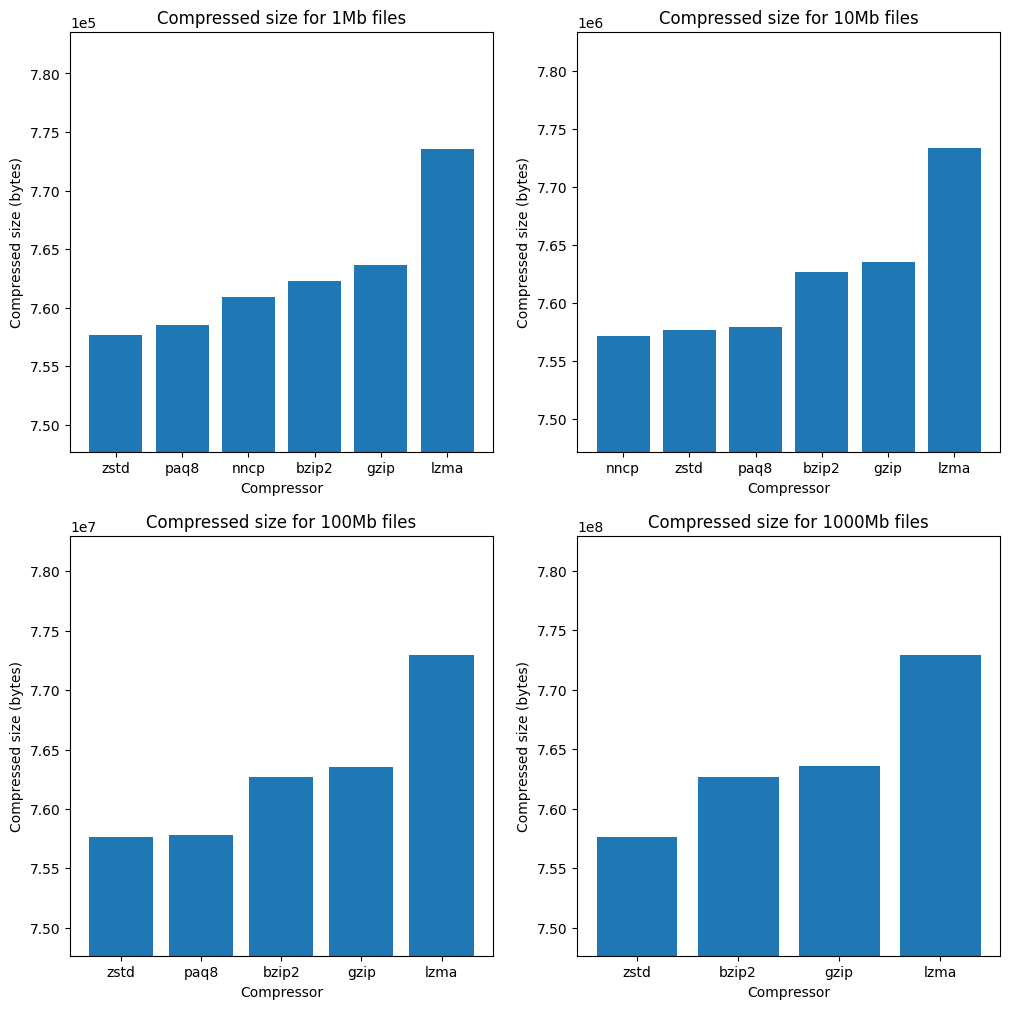
\includegraphics[width=1\textwidth]{figs/random_text_comp_size.png}
            \caption[Figure displaying the size of the compressed files generated by the general purpose algorithms when compressing random text files.] {Figure displaying the size of the compressed files generated by the general purpose algorithms when compressing random text files. Each plot is associated to one of the four text files used in the benchmark.}
            \label{fig:random_text_comp_size}
        \end{figure}

        \begin{figure}
            \centering
            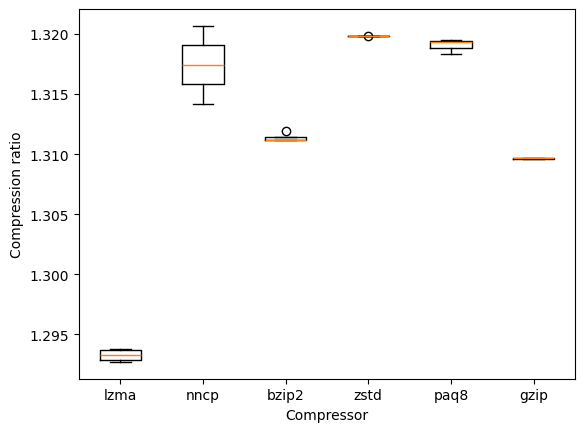
\includegraphics[width=0.5\textwidth]{figs/random_text_comp_ratio.png}
            \caption[Figure displaying the compression ratio of each general purpose compression algorithm for the random text file benchmark.] {Figure displaying the compression ratio of each general purpose compression algorithm for the random text file benchmark.}
            \label{fig:random_text_comp_ratio}
        \end{figure}

        \begin{figure}[h]
            \centering
            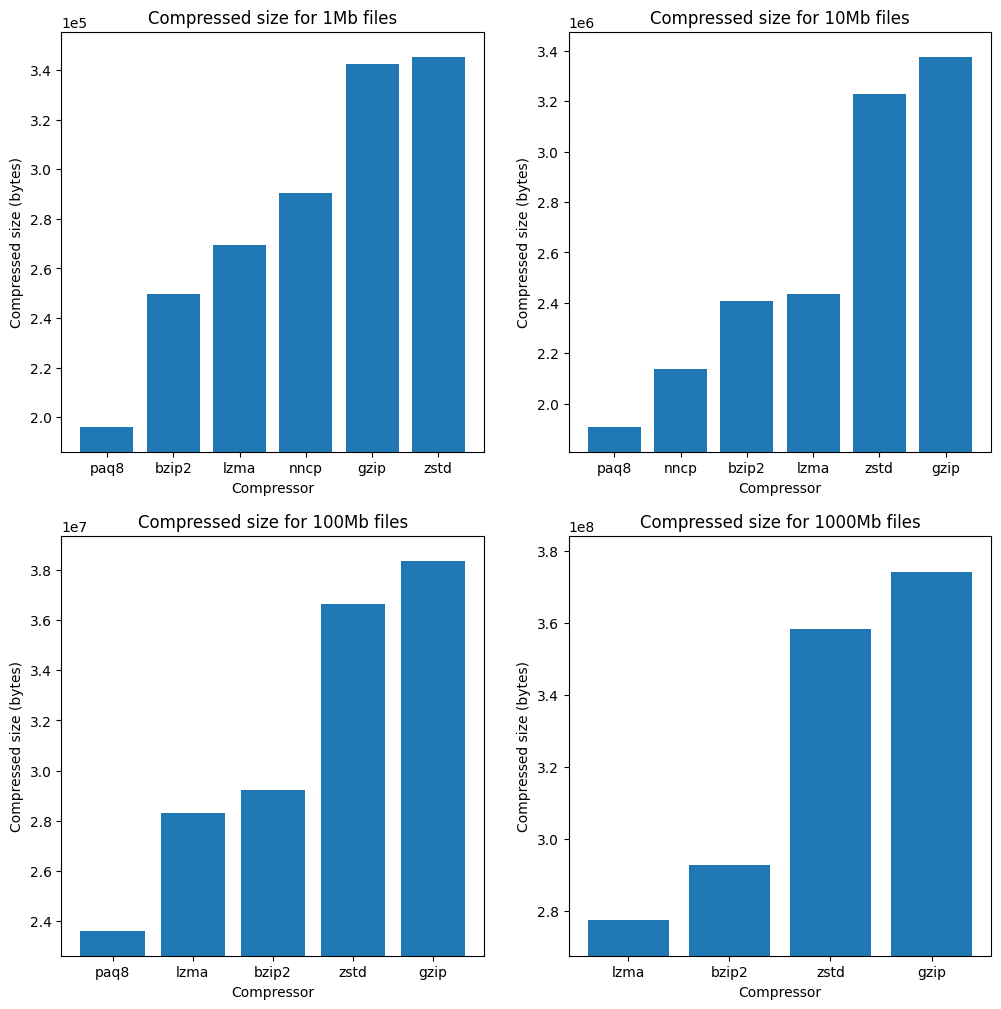
\includegraphics[width=1\textwidth]{figs/text_comp_size.png}
            \caption[Figure displaying the size of the compressed files generated by the general purpose algorithms when compressing text files.] {Figure displaying the size of the compressed files generated by the general purpose algorithms when compressing text files. Each plot is associated to one of the four text files used in the benchmark.}
            \label{fig:text_comp_size}
        \end{figure}

        \begin{figure}[h]
            \centering
            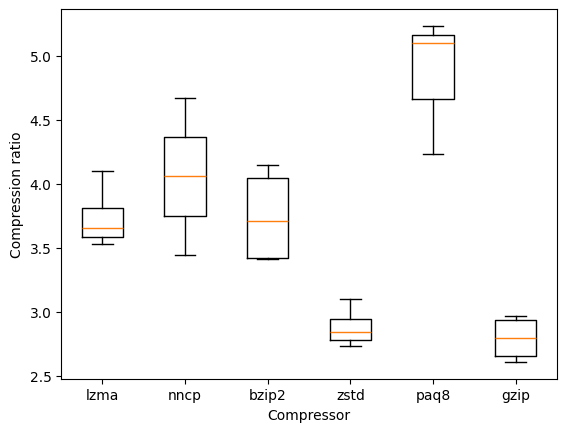
\includegraphics[width=0.5\textwidth]{figs/text_comp_ratio.png}
            \caption[Figure displaying the compression ratio of each general purpose compression algorithm for the text file benchmark.] {Figure displaying the compression ratio of each general purpose compression algorithm for the text file benchmark.}
            \label{fig:text_comp_ratio}
        \end{figure}
        
        First, we see that when dealing with random files, the compression algorithms don't have a good performance, with all algorithms having similar final compressed size, with no one having a ratio higher than 1.4. This means that if the user is expecting to receive a lot of random data, like storing binaries, using compression can be a waste of resources.
        
        Looking at the normal text results, we see that the algorithms that had the fastest metrics in the time benchmarks, \texttt{gzip} and \texttt{zstandard}, also had in general the lowest compression ratios, with both ranking as last and second to last, in almost all file sizes. This means that the algorithms that are faster are also the ones that have the worst compression ratios. This is an interesting trade-off that the user needs to consider when choosing an algorithm.
        Overall, the compression ratio of the algorithms is much better when the contents of the files aren't random, because the algorithms can find patterns in the data to compress.

        The following figures, Figures \ref{fig:text_decomp_stats} and \ref{fig:random_text_decomp_stats} show the results of the decompression metrics. We observe the same rankings as in the compression metrics, with \texttt{zstandard} being the fastest, followed by \texttt{gzip}, \texttt{bzip2} and \texttt{lzma}, and finally \texttt{paq8} being the slowest.
        The growth of the time metrics is also linear with the size of the file for all algorithms, as we can see in the figures. Due to problems with the decompression using \texttt{nncp} we had to exclude it from the benchmarks.


        \begin{figure}[h]
            \centering
            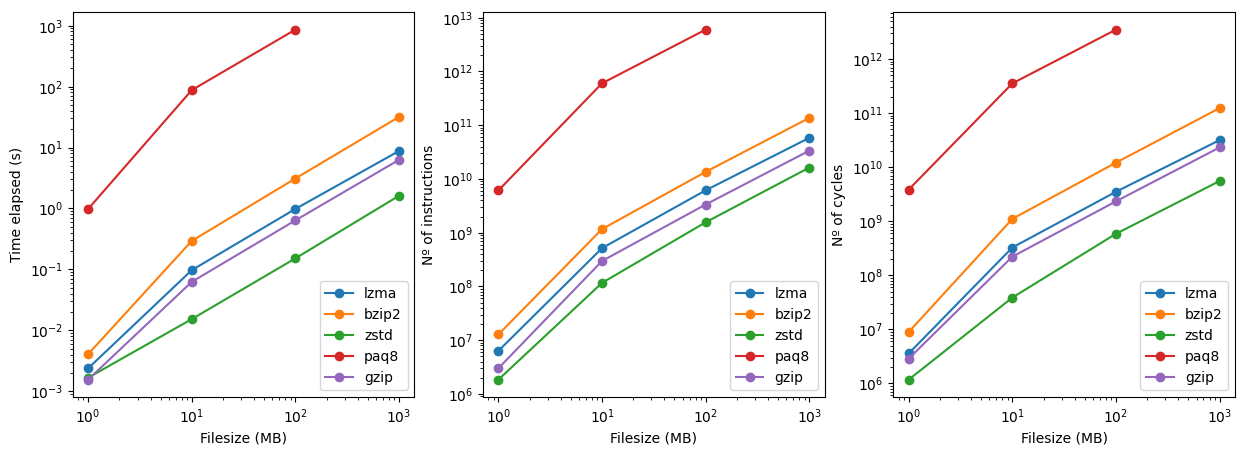
\includegraphics[width=1\textwidth]{figs/text_dstats.png}
            \caption[Figure displaying the metrics of the general purpose algorithms when decompressing text files.] {Figure displaying the metrics of the general purpose algorithms when decompressing text files. The plots display the time elapsed, the number of instructions and the number of cycles executed by the algorithms respectively.}
            \label{fig:text_dstats}
        \end{figure}

        \begin{figure}[h]
            \centering
            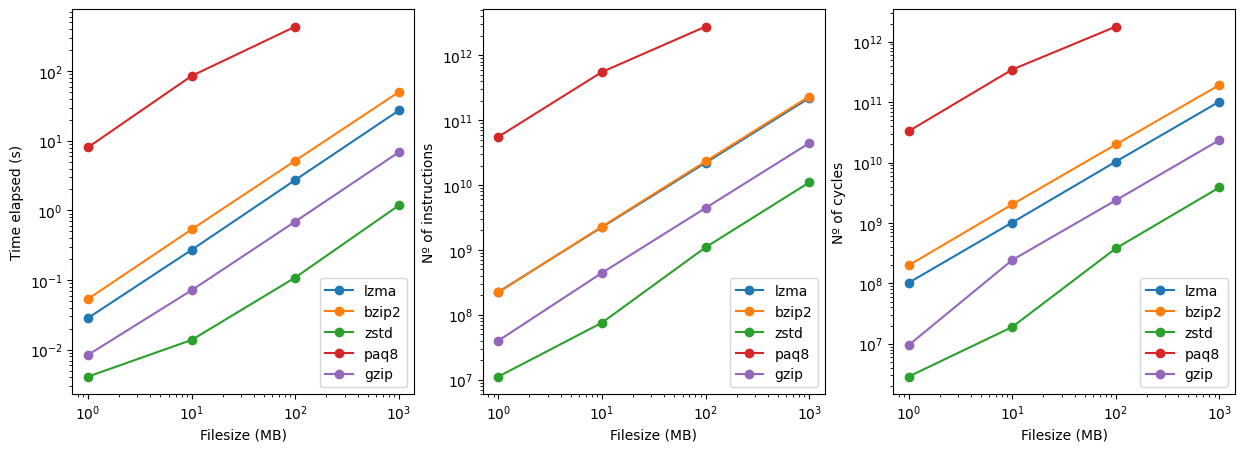
\includegraphics[width=1\textwidth]{figs/random_text_dstats.png}
            \caption[Figure displaying the metrics of the general purpose algorithms when decompressing random text files.] {Figure displaying the metrics of the general purpose algorithms when decompressing random text files. The plots display the time elapsed, the number of instructions and the number of cycles executed by the algorithms respectively.}
            \label{fig:random_text_dstats}
        \end{figure}

        With the results of these benchmarks we can determine the values for the general purpose algorithms to be used in the energy model. The values are presented in Table \ref{table:general_purpose_values}. The compression ratio is the median of the compression ratios of the algorithms in the normal text file benchmark, while the compression and decompression time costs were determined using a poly fitting algorithm to the time elapsed data of the normal and random text file benchmark.

    \begin{table}
        \caption{Values for the compression ratio, compression time cost and decompression time cost of the general purpose algorithms.}
        \label{table:general_purpose_values}
        \begin{center}
        \begin{tabular}{|| c | p{3cm} | p{3cm} | p{3cm} ||}
            \hline
            Compressor & Compression ratio $c_{ration}$ & Compression time cost $c_{t\_cost}$ & Decompression time cost $d_{t\_cost}$ \\
            \hline
            \texttt{gzip} & \multicolumn{1}{r|}{2.79} & \multicolumn{1}{r|}{\num{8.59e-2}} & \multicolumn{1}{r||}{\num{6.27e-3}} \\

            \texttt{zstandard} & \multicolumn{1}{r|}{2.89} & \multicolumn{1}{r|}{\textbf{\num{5.82e-3}}} & \multicolumn{1}{r||}{\textbf{\num{1.62e-3}}} \\

            \texttt{bzip2} & \multicolumn{1}{r|}{3.75} & \multicolumn{1}{r|}{\num{6.99e-2}} & \multicolumn{1}{r||}{\num{3.17e-2}} \\

            \texttt{lzma} & \multicolumn{1}{r|}{3.74} & \multicolumn{1}{r|}{\num{5.94e-1}} & \multicolumn{1}{r||}{\num{8.73e-3}} \\

            \texttt{paq8} & \multicolumn{1}{r|}{\textbf{4.86}} & \multicolumn{1}{r|}{\num{8.49e0}} & \multicolumn{1}{r||}{\num{8.61e0}} \\

            \texttt{nncp} & \multicolumn{1}{r|}{4.06} & \multicolumn{1}{r|}{\num{3.06e2}} & \multicolumn{1}{r||}{-} \\
            
            \hline
        \end{tabular}
        \end{center}
    \end{table}


\subsection{Specific algorithms}

    The specific algorithms were divided into two groups for each file type. The first group is the algorithms that are used to compress the genome sequence files in the FASTA format, while the second group is used to compress the genome sequence files in the FASTQ format.

    The results of the benchmarks for the genome sequence files in the FASTA format are presented in Figures \ref{fig:fasta_stats} and \ref{fig:fasta_comp_size}.
    We can see that like the general purpose algorithms, the time metrics of the specific algorithms are proportional to the size of the file, meaning that the time increase is linear with the size of the file. Also to note, that almost all algorithms had a better performance in relation to the time elapsed, than \texttt{gzip}, except for \texttt{MFCompress} which had a slight worse time.
    
    \begin{figure}[h]
        \centering
        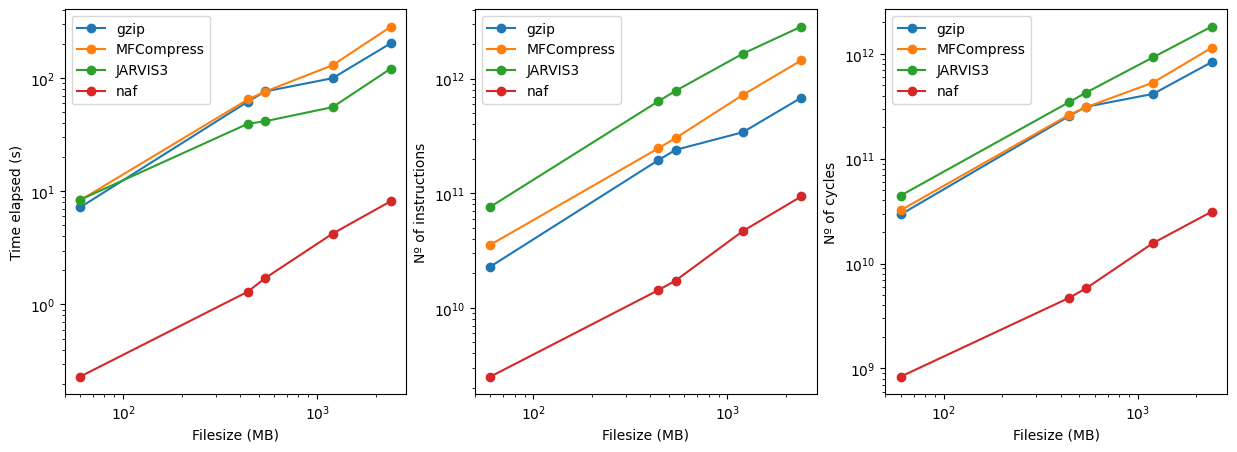
\includegraphics[width=1\textwidth]{figs/fasta_stats.png}
        \caption[Figure displaying the metrics of the specific algorithms when compressing FASTA files.] {Figure displaying the metrics of the specific algorithms when compressing FASTA files. The plots display the time elapsed, the number of instructions and the number of cycles executed by the algorithms respectively.}
        \label{fig:fasta_stats}
    \end{figure}

    \begin{figure}
        \centering
        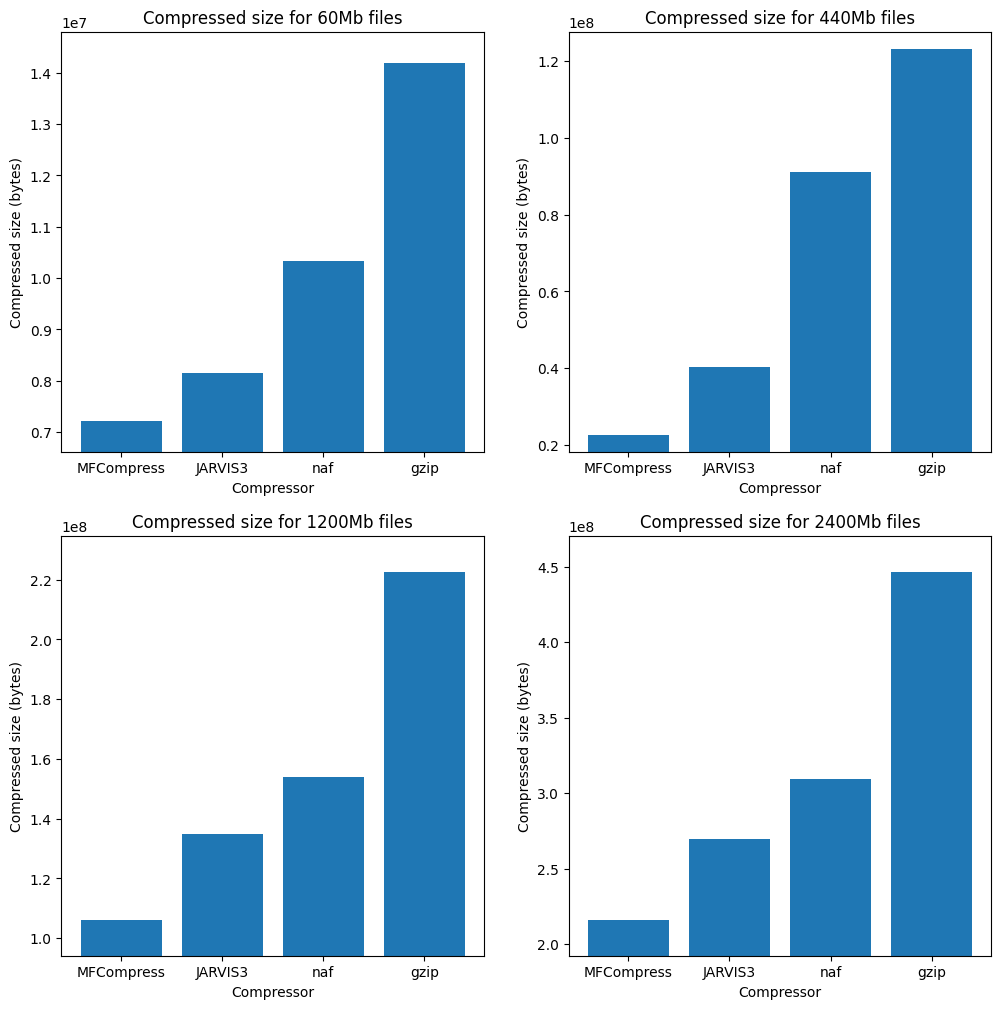
\includegraphics[width=1\textwidth]{figs/fasta_comp_size.png}
        \caption[Figure displaying the size of the compressed files generated by the specific algorithms when compressing FASTA files.] {Figure displaying the size of the compressed files generated by the specific algorithms when compressing FASTA files. Each plot is associated to one of the four text files used in the benchmark.}
        \label{fig:fasta_comp_size}
    \end{figure}

    
    In terms of compression ratio, as expected, all algorithms performed considerably better than \texttt{gzip}. There also exist a correlation with time and compression ratio, with \texttt{MFCompress} having the highest, followed by \texttt{JARVIS3}, and then \texttt{NAF}.

    For the decompression part, Figure \ref{fig:fasta_decomp_stats}, shows that like the compression metrics, the time complexity for decompression is linear with the size of the file. However, the rankings of the algorithms shifts. The new order from fastest to slowest is \texttt{NAF}, \texttt{gzip}, \texttt{JARVIS3} and \texttt{MFCompress}. There exists an irregularity in the time metrics of \texttt{MFCompress}, with the time reducing between 440MB and 540MB, this is due to the multithreading of the algorithm, which is only used when the file is larger than 500MB. 

    \begin{figure}[h]
        \centering
        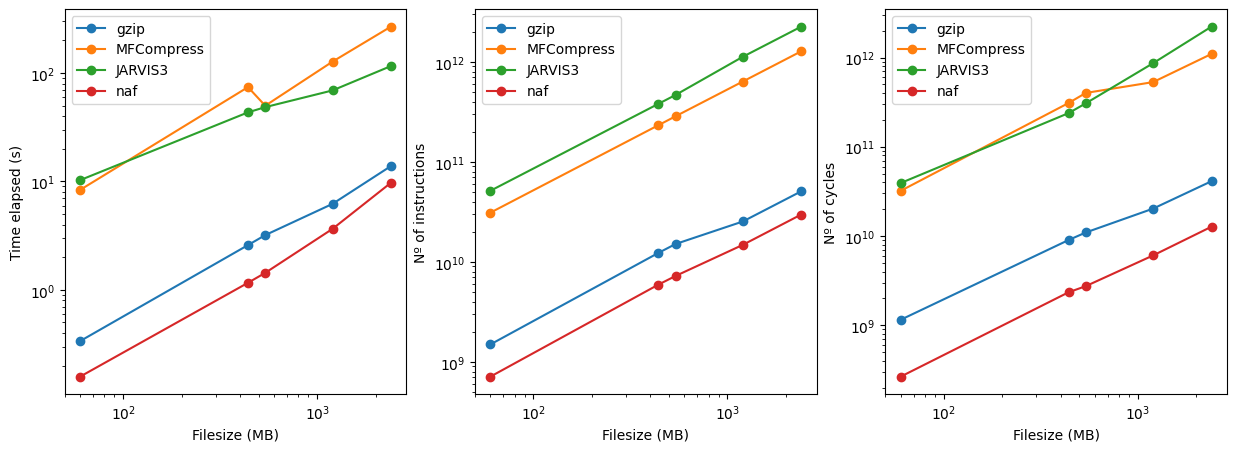
\includegraphics[width=1\textwidth]{figs/fasta_dstats.png}
        \caption[Figure displaying the metrics of the specific algorithms when decompressing FASTA files.] {Figure displaying the metrics of the specific algorithms when decompressing FASTA files. The plots display the time elapsed, the number of instructions and the number of cycles executed by the algorithms respectively.}
        \label{fig:fasta_dstats}
    \end{figure}

    The results of the benchmarks for the genome sequence files in the FASTQ format are presented in Figures \ref{fig:fastq_stats} and \ref{fig:fastq_comp_size}. Like the results for the FASTA files, most compressors presented a linear time growth, except for \texttt{spring}, more data points would be necessary to determine its growth.
    
    \begin{figure}[h]
        \centering
        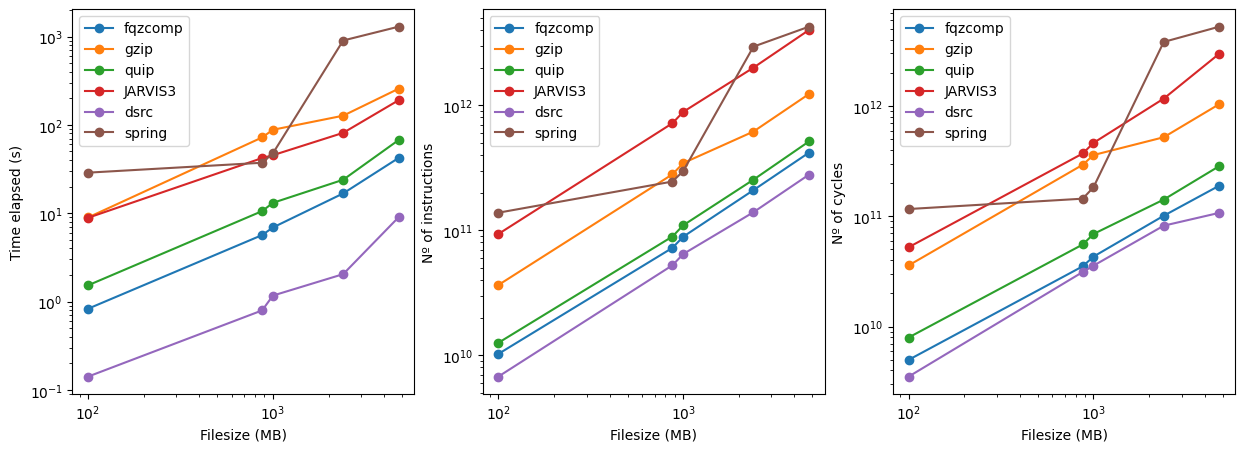
\includegraphics[width=1\textwidth]{figs/fastq_stats.png}
        \caption[Figure displaying the metrics of the specific algorithms when compressing FASTQ files.] {Figure displaying the metrics of the specific algorithms when compressing FASTQ files. The plots display the time elapsed, the number of instructions and the number of cycles executed by the algorithms respectively.}
        \label{fig:fastq_stats}
    \end{figure}

    \begin{figure}
        \centering
        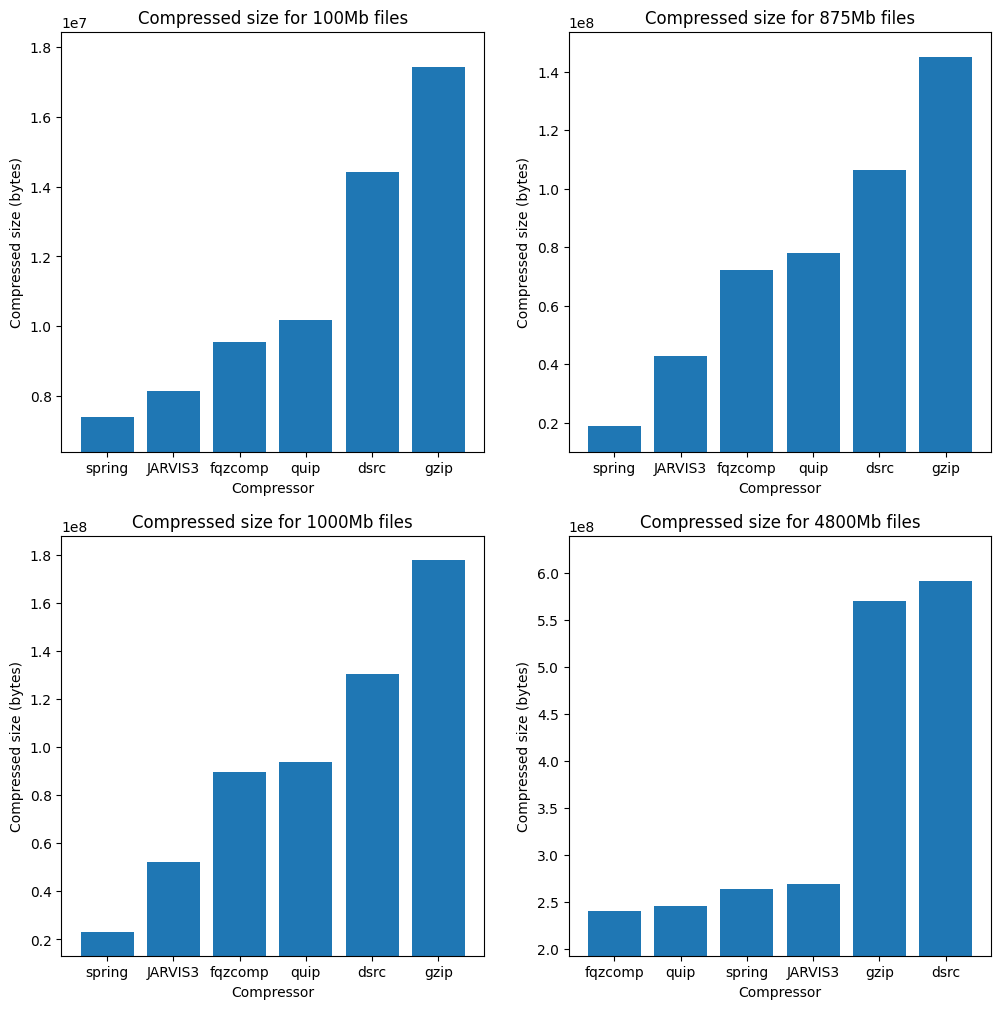
\includegraphics[width=1\textwidth]{figs/fastq_comp_size.png}
        \caption[Figure displaying the size of the compressed files generated by the specific algorithms when compressing FASTQ files.] {Figure displaying the size of the compressed files generated by the specific algorithms when compressing FASTQ files. Each plot is associated to one of the four text files used in the benchmark.}
        \label{fig:fastq_comp_size}
    \end{figure}


    The compression ratio of the specific compressors, was in general a better than \texttt{gzip}, however, \texttt{DSRC} appears to fall-off when larger files are compressed. Nonetheless, the average compression ratio of all algorithms is higher than \texttt{gzip}.

    The decompression metrics are shown in Figure \ref{fig:fastq_dstats}. In terms of time complexity, all the compressors appear to have a linear growth with the size of the file. The rankings of the algorithms also changes, with only \texttt{DSRC} performing better than \texttt{gzip}. The rest algorithms are ranked as follows, \texttt{fqzcomp}, \texttt{quip}, \texttt{spring}, and lastly \texttt{JARVIS3}.

    \begin{figure}[h]
        \centering
        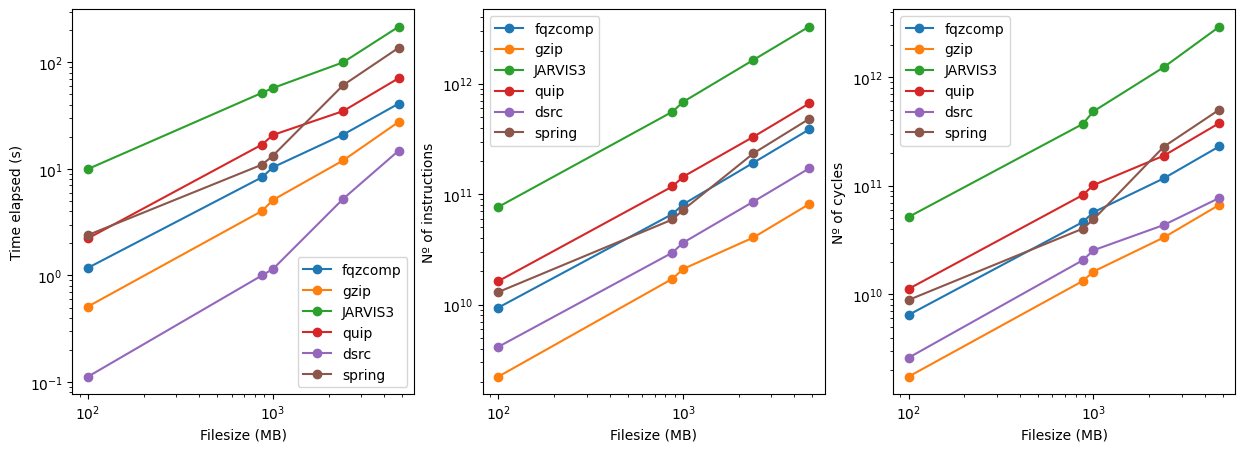
\includegraphics[width=1\textwidth]{figs/fastq_dstats.png}
        \caption[Figure displaying the metrics of the specific algorithms when decompressing FASTQ files.] {Figure displaying the metrics of the specific algorithms when decompressing FASTQ files. The plots display the time elapsed, the number of instructions and the number of cycles executed by the algorithms respectively.}
        \label{fig:fastq_dstats}
    \end{figure}


    In Table \ref{table:specific_values} we show what group each algorithm is part of, as well as the values for the compression ratio, compression time cost and decompression time cost of each compressor.


    \begin{table}
        \caption{Values for the compression ratio, compression time cost and decompression time cost of the specific compressors.}
        \label{table:specific_values}
        \begin{center}
        \begin{tabular}{|| c | c | p{3cm} | p{3cm} | p{3cm} ||}
            \hline
            Compressor & File type & Compression ratio $c_{ration}$ & Compression time cost $c_{t\_cost}$ & Decompression time cost $d_{t\_cost}$ \\
            \hline
            \texttt{gzip} & FASTA & \multicolumn{1}{r|}{4.42} & \multicolumn{1}{r|}{\num{7.72e-2}} & \multicolumn{1}{r||}{\num{5.71e-3}} \\

            \texttt{gzip} & FASTQ & \multicolumn{1}{r|}{6.85} & \multicolumn{1}{r|}{\num{4.93e-2}} & \multicolumn{1}{r||}{5e82e-3} \\

            \texttt{MFCompress} & FASTA & \multicolumn{1}{r|}{13.7} & \multicolumn{1}{r|}{\num{1.15e-1}} & \multicolumn{1}{r||}{\num{1.09e-1}} \\

            \texttt{NAF} & FASTA & \multicolumn{1}{r|}{6.20} & \multicolumn{1}{r|}{\num{3.46e-3}} & \multicolumn{1}{r||}{\num{4.16e-3}} \\

            \texttt{JARVIS3} & FASTA & \multicolumn{1}{r|}{9.44} & \multicolumn{1}{r|}{\num{4.48e-2}} & \multicolumn{1}{r||}{\num{4.416e-2}} \\

            \texttt{JARVIS3} & FASTQ & \multicolumn{1}{r|}{17.5} & \multicolumn{1}{r|}{\num{3.77e-2}} & \multicolumn{1}{r||}{\num{4.25e-2}} \\

            \texttt{DSRC} & FASTQ & \multicolumn{1}{r|}{7.81} & \multicolumn{1}{r|}{\num{1.90e-3}} & \multicolumn{1}{r||}{\num{3.28e-3}} \\

            \texttt{Fqzcomp} & FASTQ & \multicolumn{1}{r|}{14.7} & \multicolumn{1}{r|}{\num{8.92e-3}} & \multicolumn{1}{r||}{\num{8.37e-3}} \\

            \texttt{Quip} & FASTQ & \multicolumn{1}{r|}{14.1} & \multicolumn{1}{r|}{\num{1.39e-2}} & \multicolumn{1}{r||}{\num{1.41e-2}} \\

            \texttt{Spring} & FASTQ& \multicolumn{1}{r|}{27.9} & \multicolumn{1}{r|}{\num{3.07e-1}} & \multicolumn{1}{r||}{\num{3.03e-2}} \\
            
            \hline
        \end{tabular}
        \end{center}
    \end{table}


\section{Conclusions}

    The various compressors evaluated have different trade-offs between time and compression ratio. So there isn't a compressor that is the best for all scenarios, the user needs to evaluate what is more important for their use case.
    
    If the user intends to have a large cold storage, that is, a storage that is rarely accessed, the user should prioritize the compression ratio, as the time increase in compression and decompression won't be a problem. In this case, the user could opt in for the more complex algorithms, like \texttt{paq8} or \texttt{nncp}, that have the best compression ratios. 
    
    On the other hand if the user has a storage that is frequently accessed, the user should prioritize the time increase, as the user will be frequently compressing and decompressing files. In this case, the user should opt in for the faster algorithms, like \texttt{zstandard} or \texttt{gzip}. 

    Another factor to consider is the data type of the files, and use the appropriate compressor for it. Such is the case shown here of the data in the FASTA and FASTQ formats, where the specific compressors had a better performance than the general purpose compressors. 


\chapter{Web calculator - Ecompress}
\label{chapter:web_calculator}

\begin{introduction}
    This chapter explains the development of the web calculator, as well as its features and how it was implemented.

    The objective for Ecompress is to be a tool that allows the user to have a notion on the energy consumption spent by their infrastructure. It also offers the possibility to compare the efficiency of different compression algorithms to analyze which one adapts better to their use case.
\end{introduction}

\section{Solution description}

Even though the website is a simple solution, it is still crucial to define the requirements, both functional and non-functional, to ensure that the final product meets the user's expectations. 

\subsection{Functional requirements}

    \subsubsection{Parameter selection}

        The user must be able to select the parameters of the energy model to be used in the data generation process.

    \subsubsection{Data generation}

        The website must be able to generate data in accordance with the energy models studied in the previous chapter (Chapter \ref{chapter:energy_model}) and the with the own user's predefined parameters.
    
    \subsubsection{Data visualization}

        The data generated should be displayed in a clean and understandable way, so the user can easily analyze it. The user should be able to choose which graph to focus on or to display all together.

    \subsubsection{Model documentation}

        The user should have access to the documentation of the energy models used in the data generation process. This documentation should be clear and concise, so the user can understand the model's behavior and how it was implemented.

\subsection{Non-functional requirements}

    \subsubsection{Usability}
    
        The website should be intuitive to use, as well as easy to learn and understand. The platform should respect basic guidelines and best practices of web design.

    \subsubsection{Performance}

        The platform must be fast and responsive. The user should not have to wait long for the data to be generated or for the graphs to be displayed.

    \subsubsection{Security}

        User's data should be protected, and the website should be protected against common security threats.

    \subsubsection{Portability}

        The online platform should be accessible through any different web browser, regardless of the operating system or device used.

    \subsubsection{Reliability}

        The user should be able to trust the data generated and the graphs displayed.

    \subsubsection{Documentation}

        Documentation of the platform should be comprehensive and easy to understand, so as to be useful for new users.

    \subsubsection{FAIR principles}

    We also aimed to follow the FAIR principles in the development of the website. These principles are:

    \begin{itemize}
        \item Findable. The website should be easy to find, either through search engines or through direct access.
        \item Accessible. The website should be accessible to all users, regardless of their physical or cognitive abilities.
        \item Interoperable. The website should be able to interact with other systems, either through APIs or other means.
        \item Reusable. The website should be designed in a way that allows the reuse of its components in other projects.
    \end{itemize}


\subsection{System architecture}

    As we can see from the requirements, the website is a simple solution that does not require a complex system architecture, nor any complex and expensive computational resources. So the solution is a web application that uses ReactJS as the front-end framework where the data generation is handled client-side. The only server-side operation is the serving of the static files.

\section{Implementation}

    \subsection{Technology architecture}

        In terms of technologies, we used ReactJS as the main front-end framework. Then we used other libraries to handle the data visualization, the routing and the design of the website. All the libraries used are open-source and free to use and were installed using the \ac{npm}. 

    \subsubsection{ReactJS}

        ReactJS is a JavaScript library for component based front-end development. It handles the display of the \ac{DOM} elements and the management of the state of the application. 

    \subsubsection{Material-UI}

        Material-UI is a library that provides React components that implement the Material Design guidelines. It handles the design of the website, providing a clean and modern look.

    \subsubsection{better-react-mathjax}

        This library is a wrapper for the MathJax library, which allows the rendering of mathematical equations on the website.

    \subsubsection{MUI X Charts}

        This library provides React components that allow the display of different types of charts. As the name suggests, it is developed by the same team that developed Material-UI, so it integrates well with it.

    \subsubsection{React Router}

        React Router is a library that allows the handling of the routing of the website. It allows the user to navigate between different pages without the need to reload the page.

\subsection{Deployment architecture}

    The hosting of the website was done using a \ac{VM} provided by the University of Aveiro.
    Docker was used as the containerization tool to ensure that the website could be easily deployed in any environment.

\subsection{Website Structure and Functionalities}

    The website is divided into 3 main pages: the home page, the model page, and the documentation page.

    \subsubsection{Model page}

        The model page, represented in Figure \ref{fig:web_model_page}, is the main page of the website. In here, the user can visualize the energy models and select the parameters to generate the data.

        \begin{figure}[H]
            \centering
            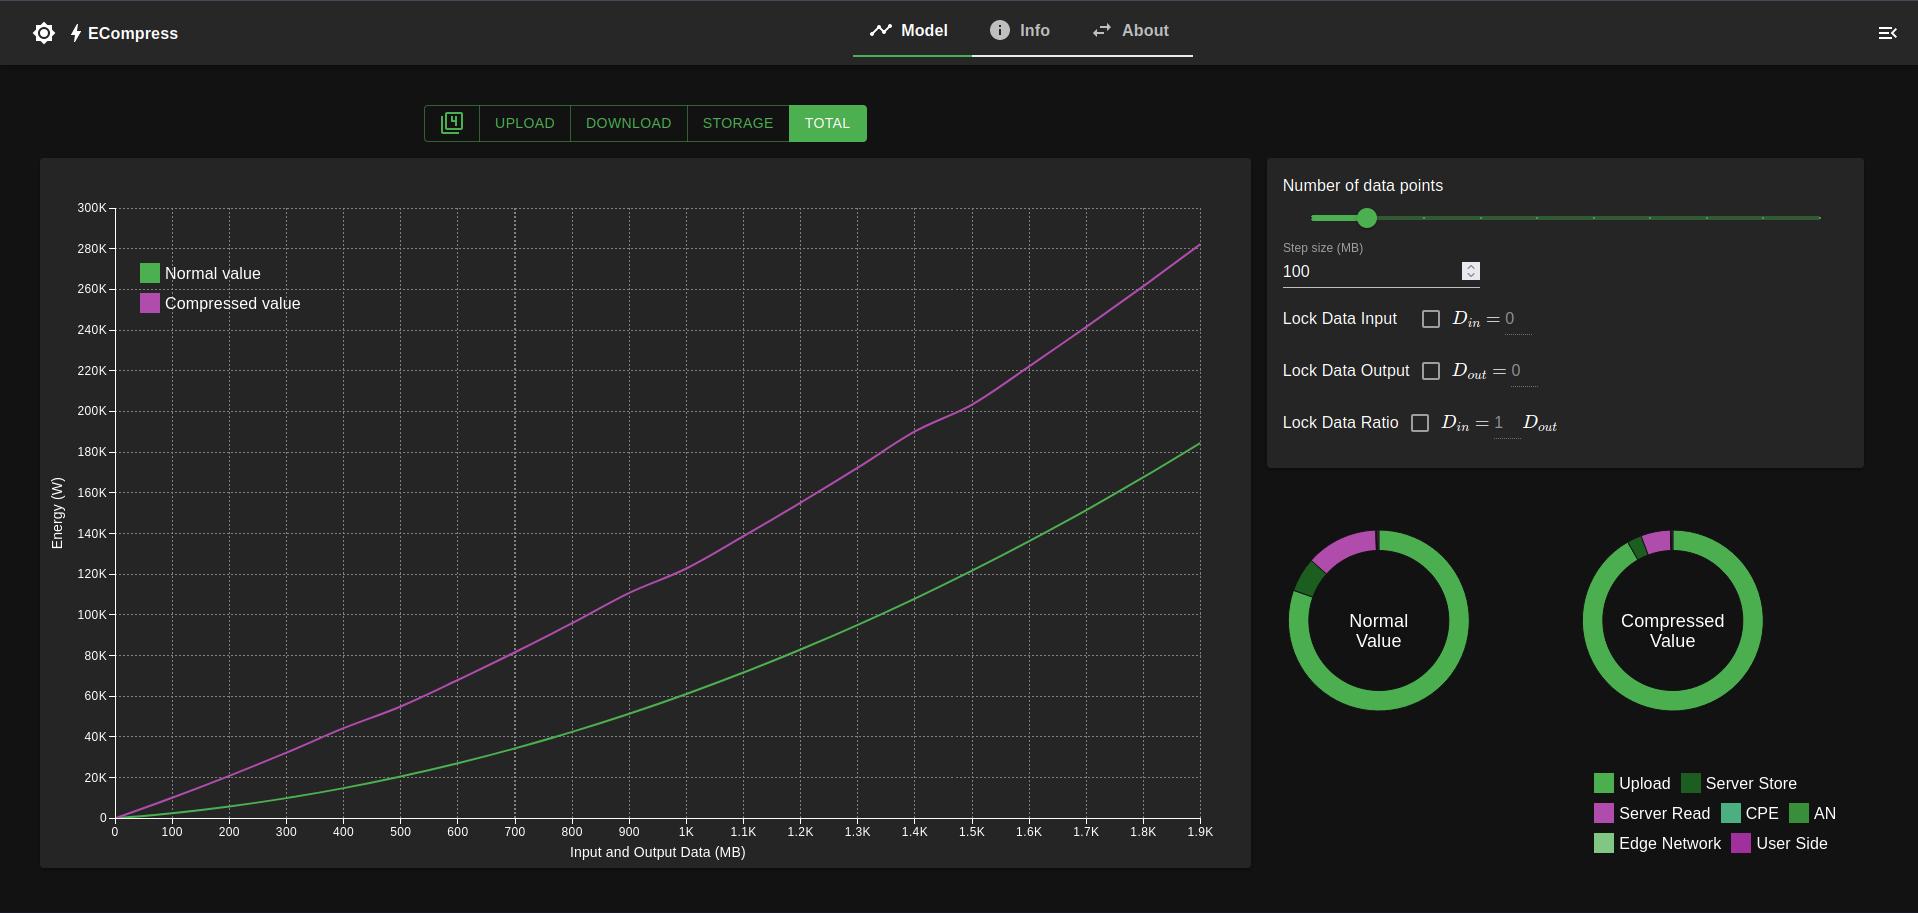
\includegraphics[width=1\textwidth]{figs/web_model_page_close.png}
            \caption{Model page of the Ecompress website.}
            \label{fig:web_model_page}
        \end{figure}

        The user can select one of 5 different visualization modes. It can be the whole energy model described in the previous chapter (chapter \ref{chapter:energy_model}), or any of the three sub-models that form the whole model, as well, as the option to show all the four models together. 

        The line chart, Figure \ref{fig:web_model_linechart}, shows two plots, one for the normal data and one for the chosen compression algorithm. The x-axis represents the size of data passing through the system, while the y-axis represents the energy consumption. In the case of the whole model, because there exists a difference between the input data (used by the upload and storage model) and the output data (used by the download model), the x-axis represents the size of both the input and output data (not cumulative). The user can select to lock one of the data types to a specific value, turning the x-axis into the variation of the other data type, or they can input a ratio between the two data types, which will split the x-axis into top and bottom, representing the output and input data sizes, respectively.
        
        \begin{figure}[H]
            \centering
            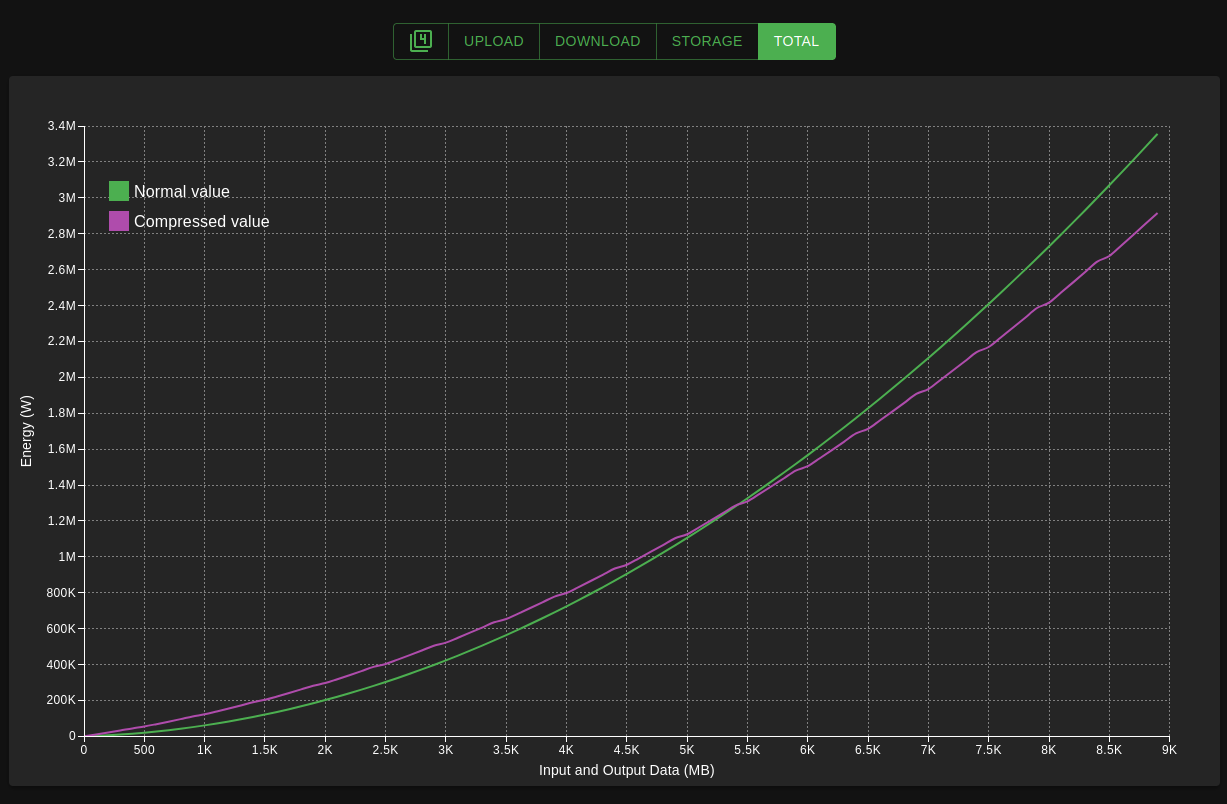
\includegraphics[width=0.8\textwidth]{figs/web_model_linechart.png}
            \caption[Line chart of the Ecompress website.] {Line chart of the Ecompress website. The green line represents the normal energy consumption, while the purple line represents the energy consumption when using a compression algorithm. On top, it shows a group of buttons to select the sub-model to be displayed.}
            \label{fig:web_model_linechart}
        \end{figure}
        
        Furthermore, the user can select any that point which will show two pie plots that show the contribution of each system component to the total energy consumption, for both the normal and compressed data. This is shown in Figure \ref{fig:web_model_piechart}.

        \begin{figure}[H]
            \centering
            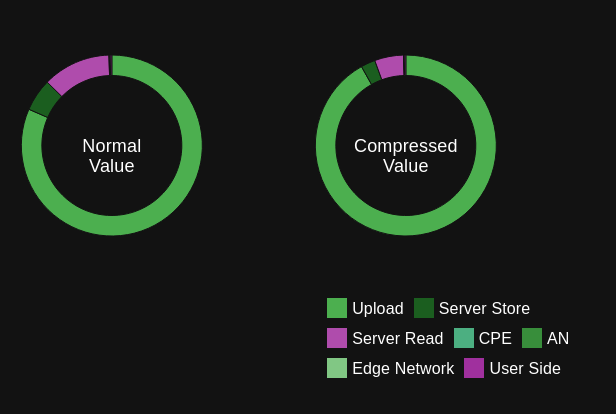
\includegraphics[width=0.6\textwidth]{figs/web_model_piechart.png}
            \caption[Pie chart of the Ecompress website.] {Pie chart of the Ecompress website. The left pie represents the normal energy consumption, while the right pie represents the energy consumption when using a compression algorithm.}
            \label{fig:web_model_piechart}
        \end{figure}

        It is also provided the ability to select the number of data points to be generated, as well as the time interval between each data point.

        To change the parameters, the user can click on the drawer open button, which will change the layout of the page to show side by side the graph and the form, as shown in Figure \ref{fig:web_calculator_drawer_open}. To return to the previous view, the user can click the same button, which will close the drawer.

        \begin{figure}[H]
            \centering
            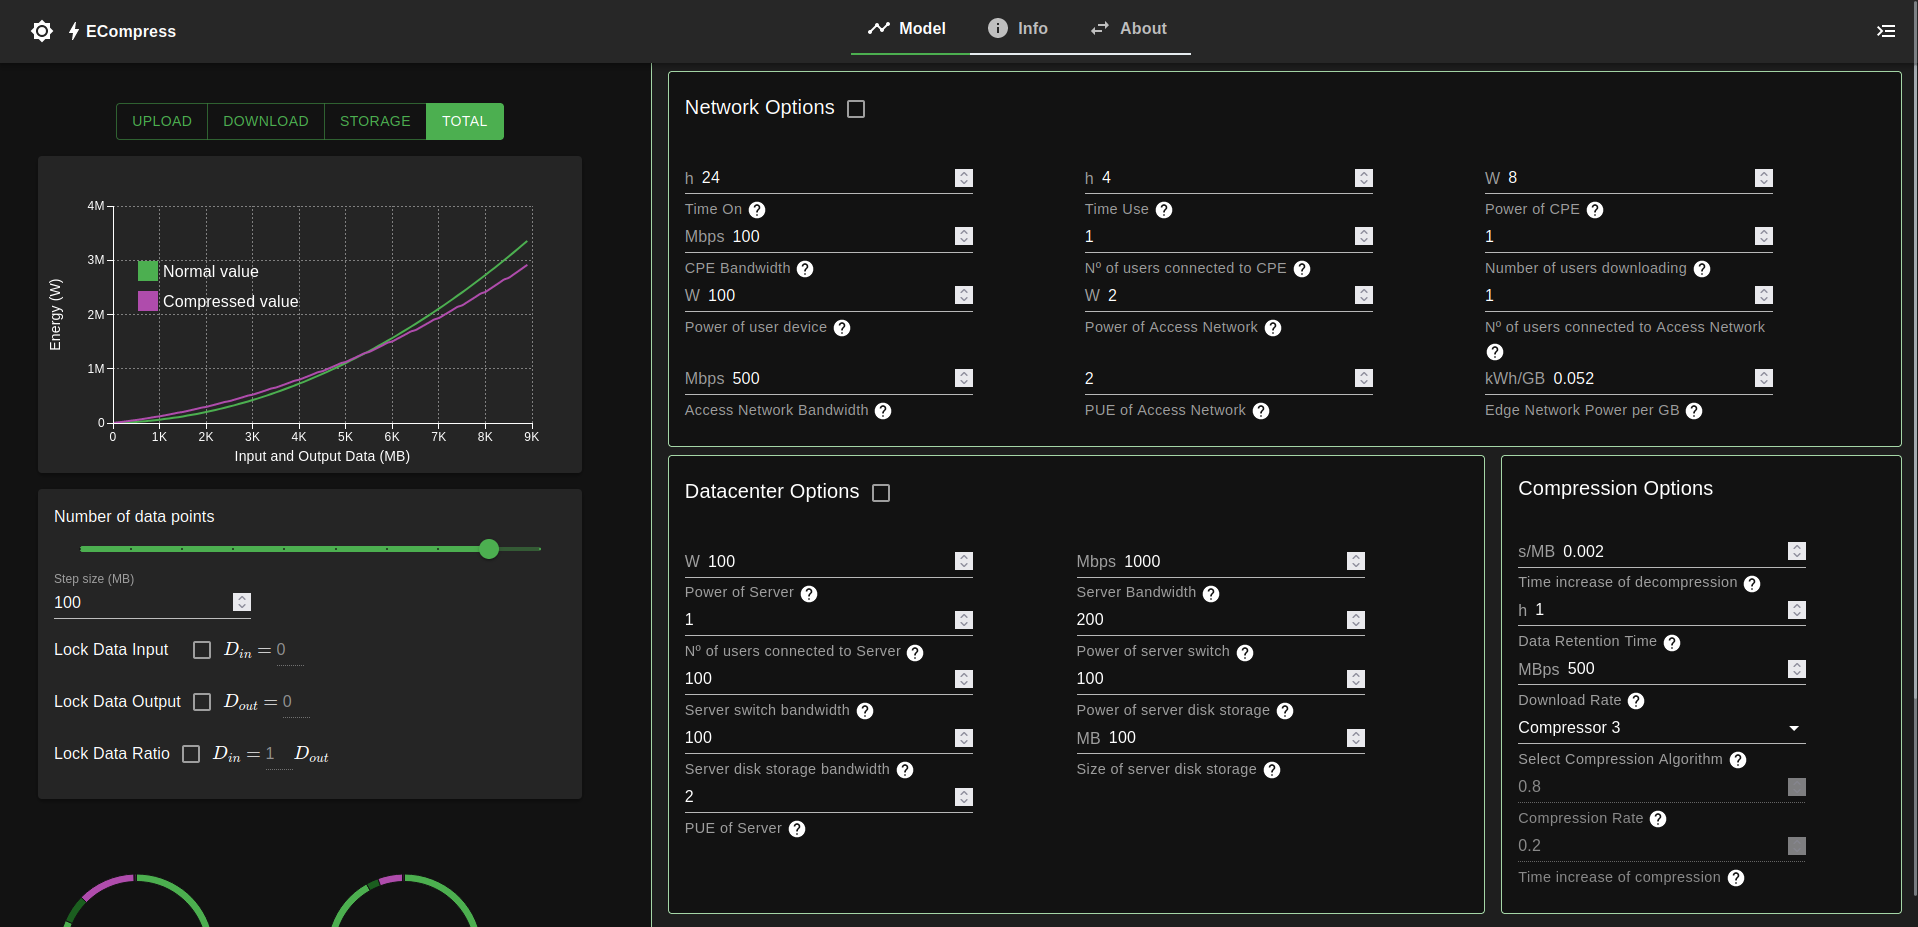
\includegraphics[width=1\textwidth]{figs/web_model_page_open.png}
            \caption[Model page of the Ecompress website with the drawer open.]{Model page of the Ecompress website with the drawer open. The contents of the graph are moved to the right, occupying one third of the screen, while the form is shown on the left, occupying two thirds of the screen.}
            \label{fig:web_calculator_drawer_open}
        \end{figure}

        The form is divided by each system component, and the user needs to submit with valid inputs for the data generation to start. The website doesn't provide an account option to save the user's preferences, however local storage is used to save the last parameters used by the user. 

    \subsubsection{Info page}

        The Info page (figure \ref{fig:info_page}) is a simple documentation page that explains how the energy models work, exposing the mathematical equations behind each graph.

        \begin{figure}[H]
            \centering
            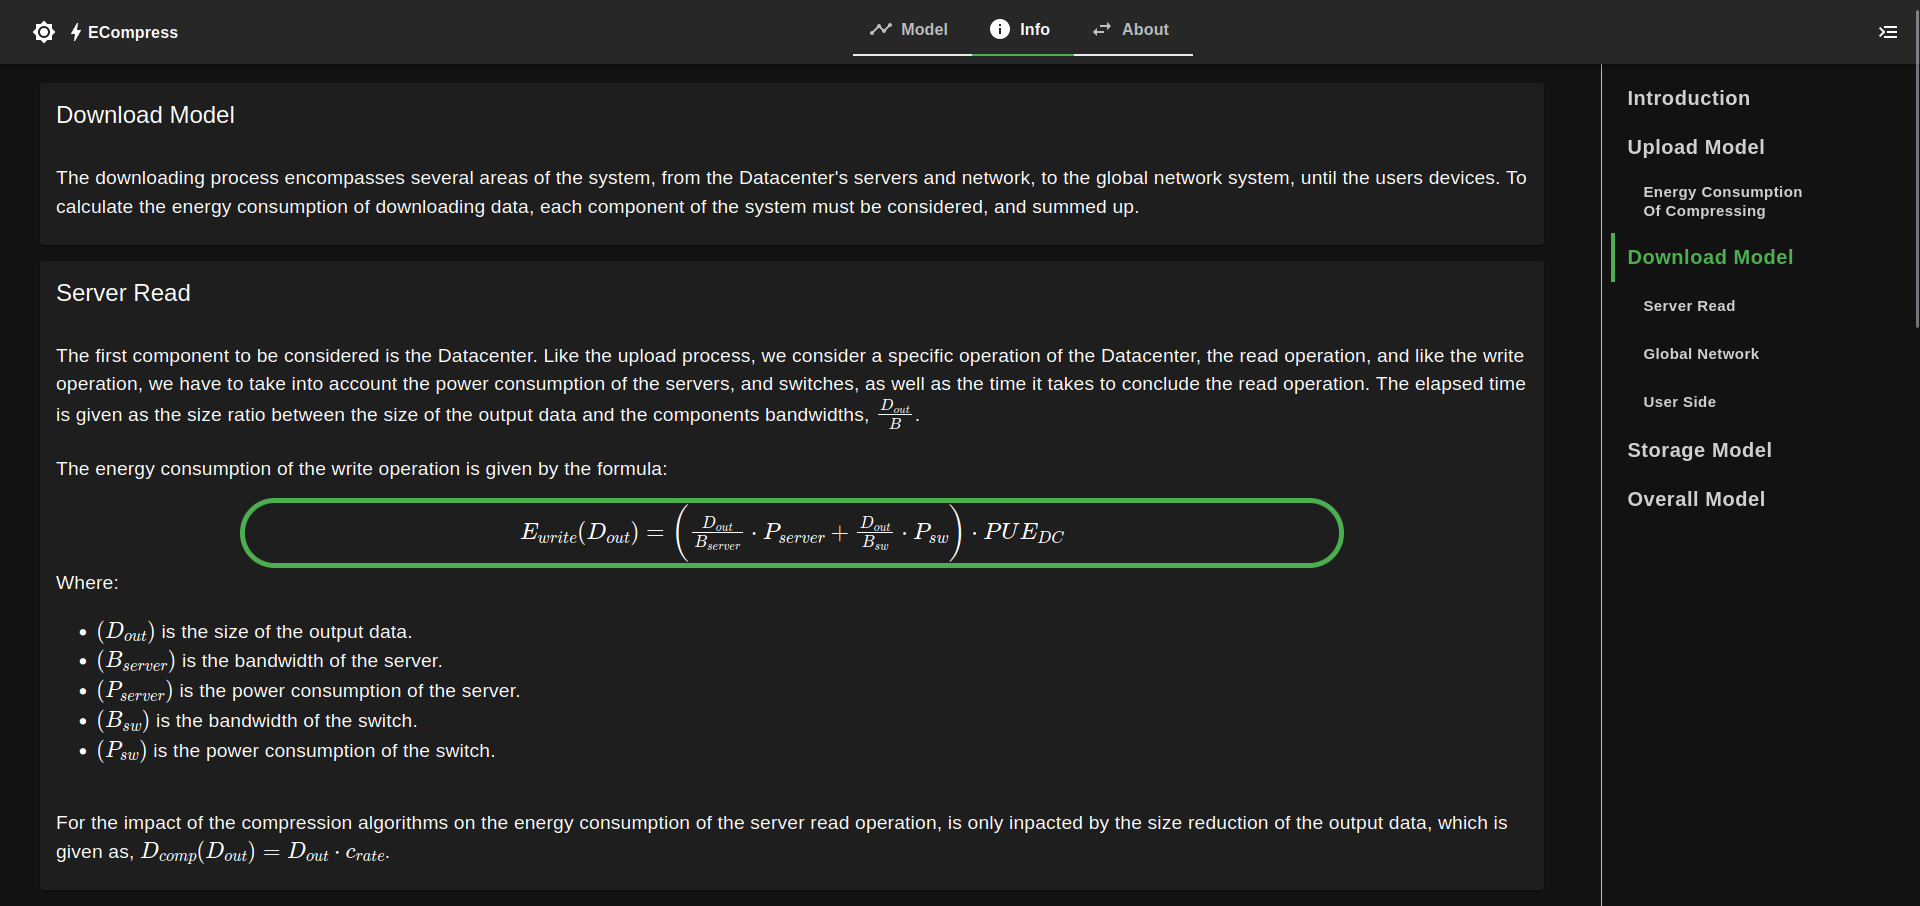
\includegraphics[width=1\textwidth]{figs/web_info_page.png}
            \caption{Information page of the Ecompress website.}
            \label{fig:info_page}
        \end{figure}

        The page is divided into several sub-pages that can be navigated through the sidebar which like the model can be collapsed for a fuller view of the content.

    \subsubsection{About page}

        The About page (figure \ref{fig:about_page}) shows information about the project, the authors and the institution behind the project. 


%%%%%%%%%%%%%%%%%%%%%%%%%%%%%%%%%%%%%%%%%%%%%%%%%%%%%%%
% End of Thesis text 
%%%%%%%%%%%%%%%%%%%%%%%%%%%%%%%%%%%%%%%%%%%%%%%%%%%%%%%

\backmatter

%%%%%%%%%%%%%%%%%%%%%%%%%%%%%%%%%%%%%%%%%%%%%%%%%%%%%%%
% Print all used references
%%%%%%%%%%%%%%%%%%%%%%%%%%%%%%%%%%%%%%%%%%%%%%%%%%%%%%%

\begingroup
\renewcommand{\bibfont}{\footnotesize}
% Redefine References name to Portuguese
% Change if you are using english
\defbibheading{bibliography}[References]{
	\chapter{#1}
}
\SingleSpacing
\setlength\bibitemsep{8pt}
\printbibliography[heading=bibliography]
\endgroup


%%%%%%%%%%%%%%%%%%%%%%%%%%%%%%%%%%%%%%%%%%%%%%%%%%%%%%%
% Load appendix
%%%%%%%%%%%%%%%%%%%%%%%%%%%%%%%%%%%%%%%%%%%%%%%%%%%%%%%

\mainmatterWithoutReset
\appendix

% \chapter{Additional content}


\end{document}
